\documentclass[twoside,11pt]{homework}

\coursename{COMS 4771 Machine Learning 2020} 

\studname{Joseph High, Eliza Mace, Zachary Schuermann}
\studmail{jph2185, emm2314, zvs2002}
\hwNo{2}
\date{\today} 

% Uncomment the next line if you want to use \includegraphics.
\usepackage{graphicx}
%\usepackage{fancyhdr}
\usepackage{enumerate}
\usepackage{amsmath}
\usepackage{relsize}
\usepackage{mathtools}
\usepackage{dsfont}
\usepackage[dvipsnames]{xcolor}
\usepackage[makeroom]{cancel}
\usepackage{collectbox}
\usepackage{placeins}

\DeclarePairedDelimiter{\2norm}{\lVert}{\rVert^2_2}
\newcommand{\defeq}{\vcentcolon=}
\newcommand\unif{\ensuremath{\operatorname{unif}}}
\DeclareMathOperator{\EX}{\mathbb{E}}% expected value
\newcommand{\1}[1]{\mathds{1}\left[#1\right]}

\makeatletter
\newcommand{\mybox}{%
    \collectbox{%
        \setlength{\fboxsep}{1pt}%
        \fbox{\BOXCONTENT}%
    }%
}

%%%%%%%%%%%%%%%% Direct Comments %%%%%%%%%%%%%%%%
\newcommand{\joe}[1]{\textcolor{yellow}{\colorbox{blue}{\parbox{15.5cm}{\textbf{\textsc{Joe}: \ #1}}}}}
%newcommand{\joe}[1]{}
\newcommand{\eliza}[1]{\textcolor{black}{\colorbox{cyan}{\parbox{15.5cm}{\textbf{\textsc{Eliza}: \ #1}}}}}
%newcommand{\eliza}[1]{}
\newcommand{\zach}[1]{\textcolor{blue}{\colorbox{gray}{\parbox{15.5cm}{\textbf{\textsc{Zach}: \ #1}}}}}
%newcommand{\zach}[1]{}
%%%%%%%%%%%%%%%%%%%%%%%%%%%%%%%%%%%%%%%%%%%%%%%%%

\begin{document}
\maketitle

\section*{Problem 1: A variant of Perceptron Algorithm}
Given our Perceptron OR Variant with binary observations from a $d$-dimensional
feature space, ($x \in \{0, 1\}^{d}$) and output defined as an `OR' of some of the
features, we can show it makes at most $2 + 3r(1+\log d)$ mistakes when the
target concept is an OR of $r$ variables.
\begin{enumerate}[\bf (i)]   
	\item
	We can show that the Perceptron OR Variant makes $M_{+}\leq r(1+ \log d)$
	mistakes on positive examples:
	first consider the worst scenario in which positive mistakes are made. It
	can be observed that the algorithm will make the most mistakes when a vector
	with a single 1 element is given for the weights which has the weight of
	that element assigned to 1.
	
	As a example for intuition, we can consider the case when $d = 4$, given
	an $x_{i}=[1,0,0,0]$ predicted positively ($x_{0}$ is one of the terms in
	the target OR) we know that in order for the algorithm to predict positively
	for $x_{i}$, it must iterate the following weights:  \\ \\
	start: $w = [1,1,1,1]$
	\begin{enumerate}[(1)]
		\item
		$w = [2,1,1,1]$
		\item
		$w = [4,1,1,1]$
		\item
		$w = [8,1,1,1]$
	\end{enumerate}
	Notice that the algorithm will make $1 + \log d$ mistakes until the element
	$w_{i}$ exceeds $d$ (the requirement to successfully label $x_{i}$). Since
	this can occur for each of the terms in the target OR, there are $r$ such
	instances above; meaning, there are at most $r(1 + \log d)$ mistakes for any
	positive example.
	
	\item
	Similar to the part above, we will consider the ``boundary'' case to provide
	a lower bound on the decrease in the total weight $\sum_{i}w_{i}$.
	In order for the algorithm to incorrectly classify a negative example, we
	have:
	\[
	\hat{y} = 1 , y = 0
	\]
	Since $\hat{y} = \1{w \cdot x > d} = 1$, we have:
	\[
	1 = \1{w \cdot x > d}
	\implies w \cdot x > d
	\]
	Above, we have shown that each mistake made on a negative example is
	predicated on: $ w \cdot x > d$. With this observation, we can prove a lower
	bound on the decrease in the total weight after the algorithm's update.
	First, consider we can rewrite:
	\[
	w \cdot x > d
	\]
	as
	\[
	\sum_{i}w_{i} (\forall i : x_{i} = 1) > d.
	\]
	After performing the update:
	$w_i \leftarrow w_{i}/2 (for \forall i : x_{i} = 1)$, we can see that every
	term in the summation above is updated (divided by two) since they are
	predicated on the same expression. We have the following for the old
	$w_{i}$'s:
	\[
	\frac{1}{2}\sum_{i}w_{i} (\forall i : x_{i} = 1) > \frac{d}{2}.
	\]
	And since the new $w_{i}$'s are given by:
	\[
	\frac{1}{2}\sum_{i}w_{i} (\forall i : x_{i} = 1)
	\],
	For the new $w_{i}$'s we have:
	\[
	\sum_{i}w_{i} (\forall i : x_{i} = 1) > \frac{d}{2}
	\]
	We can effectively drop the predicate since $\sum_{i}w_{i} \geq
	\frac{1}{2}\sum_{i}w_{i} (\forall i : x_{i} = 1)$. This yields:
	\[
	\sum_{i}w_{i}  > \frac{d}{2}.
	\]
	Thus, the updated weights at each negative mistake are decreased by at least
	$\frac{d}{2}$.
	
	%\end{align*}
	\item
	Let $M_{-}$ denote the total number of mistakes on negative examples, and
	$TW(t)$ denote the total weight of $w$ at iteration $t$. Observe that
	\[
	0 < TW(t) \leq TW(0) + dM_{+} - (d/2)M_{-}.
	\]
	
	First, we can prove that
	\[
	TW(t) \leq TW(0) - \frac{d}{2}M_{-}
	\]
	since there are $M_{-}$ total negative mistakes and each decreases the total
	weight by at least $\frac{d}{2}$, the total weight at iteration $t$ must be at most the
	difference between the initial weight ($TW(0)$) and the accumulated changes
	to the weights since $t=0$, $(d/2)M_{-}$.
	
	Similarly, we can prove
	\[
	TW(t) \leq TW(0) + dM_{+}.
	\]
	First, consider the most that each mistake on a positive example can
	increase the total weight $\sum_{i}w_{i}$. Similar to (ii), we first
	predicate on $\hat{y} = 0, y = 1$.
	Since $\hat{y} = \1{w \cdot x > d} = 0$, we have:
	\[
	0 = \1{w \cdot x > d}
	\implies w \cdot x \leq d
	\]
	Then,
	\[
	\sum_{i}w_{i} (\forall i : x_{i} = 1) \leq d.
    \]
In a similar vein as above, at each iteration in the algorithm, the update
    cannot exceed an addition of $d$ to the total weight, since anytime
    element's corresponding weight is updated, it must be less than or equal to
    $d$ (meaning the update from $d$ to $2d$ is in fact the maximum - which is
    simply $d$).

	Finally, we will rearrange the original observation and use
	$M_{+} \leq r(1+\log d)$:
	\begin{align*}
	0 &< TW(t) \leq TW(0) + dM_{+} - (d/2)M_{-} \\
	\frac{d}{2}M_{-} &< TW(t) + \frac{d}{2}M_{-} \leq TW(0) + dM_{+} \\
	\intertext{dropping the middle term:} \\
	\frac{d}{2}M_{-} &\leq TW(0) + dM_{+} \\
	M_{-} &\leq \frac{2}{d}\left(TW(0) + dM_{+}\right) \\
	M_{-} &\leq \frac{2}{d}\left(d + dM_{+}\right) \\
	M_{-} &\leq 2 + 2M_{+} \\
	M_{-} &\leq 2 + 2(r (1 + \log d)) \\
	M_{-} &\leq 2 + 2r + 2r\log d \\
	\end{align*}
	
	Now that we have bounds on both $M_{-}$ and $M_{+}$, we can establish a
	bound on the total number of mistakes:
	\begin{align*}
	M_{+} + M_{-} &\leq r(1+\log d) + 2 + 2r + 2r\log d \\
	M_{+} + M_{-} &\leq r + r\log d + 2 + 2r + 2r\log d \\
	M_{+} + M_{-} &\leq 2 + 3r + 3r\log d \\
	M_{+} + M_{-} &\leq 2 + 3r(1 + \log d) \\
	\end{align*}
	
	Thus, we can conclude that the total number of mistakes ($M_{+} + M_{-}$) is
	at most $2 + 3r(1 + \log d)$.
	
\end{enumerate}

\section*{Problem 2: Inconsistency of the fairness definition}

\begin{enumerate}[\bf (i)]
	
	\item Only trivial scenarios are able to satisfy all three fairness definitions simultaneously. Consider the problem of hiring (``hire'' vs. ``do not hire'') where the sensitive attribute is gender (``male'' vs. ``female''). In this case, if there are an equal number of male and female candidates, and they are hired at exactly equal rates (and we have a perfect classifier), then all three fairness definitions can be satisfied. The number of men and number of women must be the same, as well as the number of men hired and the number of women hired.
	
	\item Demographic Parity tells us that:
	\begin{equation}
	\mathbb{P}_0[\hat{Y}=\hat{y}]=\mathbb{P}_1[\hat{Y}=\hat{y}]
	\end{equation}
	This implies that the predicted class is independent of the sensitive attribute:
	\begin{equation}
	\hat{Y}\perp A
	\end{equation}
	and by the symmetry property of conditional independence:
	\begin{equation}
	\label{eqn:dp}
	A \perp \hat{Y}
	\end{equation}
	On the other hand, Predictive parity is defined as:
	\begin{equation}
	\mathbb{P}_0[Y=y|\hat{Y}=\hat{y}]=\mathbb{P}_1[Y=y|\hat{Y}=\hat{y}]
	\end{equation}
	Which tells us that the sensitive attribute is independent of the true class, given the predicted class:
	\begin{equation}
	A \perp Y|\hat{Y}
	\end{equation}
	Thus, if $A \not\perp Y$,
	\begin{equation}
	A \not\perp \hat{Y}
	\end{equation}
	which contradicts equation \ref{eqn:dp}, showing that Demographic Parity and Predictive Parity cannot both hold if $A \not\perp Y$.
	\item As in part (ii), demographic parity gives that:
	\begin{equation}
	\label{eqn:dp2}
	\hat{Y} \perp A
	\end{equation}
	The Equalized Odds fairness metric says that the predicted class is independent of the sensitive attribute, given the true class:
	\begin{equation}
	\label{eqn:eo}
	\hat{Y} \perp A | Y
	\end{equation}
	By contraction:
	\begin{equation}
	\hat{Y} \perp A,Y
	\end{equation}
	Then by decomposition:
	\begin{equation}
	\hat{Y} \perp A
	\end{equation}
	AND
	\begin{equation}
	\hat{Y} \perp Y
	\end{equation}
	For both equations to be true, either the sensitive attribute OR the predicted class must be independent of the actual class:
	\begin{equation}
	A\perp Y
	\end{equation}
	OR
	\begin{equation}
	\hat{Y}\perp Y
	\end{equation}
	Thus, if $A\not\perp Y$ and $\hat{Y}\not\perp Y$, both Demographic Parity (\ref{eqn:dp2}) and Equalized Odds (\ref{eqn:eo}) cannot hold at the same time.
	\item As shown in part (ii), when Equalized Odds holds:
	\begin{equation}
	\hat{Y} \perp A|Y
	\end{equation}
	Which gives us that:
	\begin{equation}
	\label{eqn:eo2}
	A\perp \hat{Y}|Y
	\end{equation}
	And from part (i), the definition of Predictive Parity is:
	\begin{equation}
	Y\perp A|\hat{Y}
	\end{equation}
	Which tells us:
	\begin{equation}
	\label{eqn:pp2}
	A\perp Y|\hat{Y}
	\end{equation}
	Combining equations \ref{eqn:eo2} and \ref{eqn:pp2} gives:
	\begin{equation}
	A\perp Y,\hat{Y}
	\end{equation}
	By decomposition, $A \perp Y$, so if we are given $A \not\perp Y$, both Equalized Odds and Predictive Parity cannot hold.
\end{enumerate}


\section*{Problem 3: Making data linearly separable by feature space mapping}

\begin{enumerate}[\bf (i)]

\item 
\begin{proof}
We are given that $$\Phi_{\alpha}(x_i) = \begin{cases} \mathlarger{\text{exp}\left(-\frac{1}{1-(\frac{\alpha-x_i}{\sigma})^2}\right)} \ , & |\alpha - x_i| < \sigma \\ 0 \ ,& \text{otherwise} \end{cases}$$


Because we are only concerned with a finite number of data points, $x_1 \dots , x_n$, there exists some $\varepsilon > 0$ such that $|x_i - x_j| > \varepsilon$ for all $i, j \in \{1, \dots, n\}$. Then, we have that $\varepsilon < \min_{i,j}|x_i - x_j|$. Using this fact, set $\mathlarger{\sigma = \frac{\varepsilon}{2}}$ so that for any $x_i$ and $x_j$, where $x_i \neq x_j$, we have
$$\int_{-\infty}^{\infty} \Phi_{\alpha}(x_i)\Phi_{\alpha}(x_j)d\alpha = \int_{x_i-\sigma}^{x_i + \sigma}\Phi_{\alpha}(x_i)\Phi_{\alpha}(x_j)d\alpha = 0$$

Define our classifier to be such that $ \ \text{sign}(w_i \Phi_{\alpha}(x_i)) = y_i , \ \forall i \in \{1, \dots, n\}$.  \\ 
Then set $\mathlarger{\vec{\bf w} = \sum_{k=1}^n w_k y_k \Phi_{\alpha}(\vec{x_k})}$. We then have the following:
\begin{align*}
\text{sign}\left(\vec{\bf w}\cdot \Phi_{\alpha}(\vec{x_i})\right) & =  \text{sign}\left(\Phi_{\alpha}(\vec{x_i}) \cdot \sum_{k=1}^n w_k y_k \left(\Phi_{\alpha}(\vec{x_k})\right)\right)  \\
& = \text{sign}\left(\int_{x_i-\sigma}^{x_i + \sigma}\sum_{k=1}^n w_k y_k \Phi_{\alpha}(\vec{x_k}) \Phi_{\alpha}(\vec{x_i})d\alpha\right) \\
& = \text{sign}\left(w_i y_i\int_{x_i-\sigma}^{x_i + \sigma}\Phi_{\alpha}(\vec{x_i}) \Phi_{\alpha}(\vec{x_i})d\alpha\right) \\
& = \text{sign}\left(w_i y_i\int_{x_i-\sigma}^{x_i + \sigma}\Phi_{\alpha}(\vec{x_i})^2d\alpha\right) = y_i
\end{align*}

\end{proof}

\item For arbitrary $x$ and $x'$, we want to express the dot product analytically. We have two cases: (1) $x \neq x '$ , and (2) $x = x'$.  \\

\underline{Case 1 ($x \neq x '$)}:

From part (i) we have the following for any two distinct points:
$$\Phi_{\alpha}(x) \cdot \Phi_{\alpha}(x) = \int_{-\infty}^{\infty} \Phi_{\alpha}(x) \Phi_{\alpha}(x') d\alpha \ = \ 0$$


\underline{Case 2 ($x = x '$)}:
\begin{align*}
\Phi_{\alpha}(x) \cdot \Phi_{\alpha}(x) & = \int_{-\infty}^{\infty} \Phi_{\alpha}(x) \Phi_{\alpha}(x') d\alpha \\ & = \int_{-\infty}^{\infty} \Phi_{\alpha}(x)^2 d\alpha \\
& = \int_{x-\sigma}^{x+\sigma} \mathlarger{\left(e^{-\mathlarger{\frac{1}{1-(\frac{\alpha-x}{\sigma})^2}}}\right)^2} d\alpha \\
& = \int_{x-\sigma}^{x+\sigma} \mathlarger{e^{-\mathlarger{\frac{2}{1-(\frac{\alpha-x}{\sigma})^2}}}} d\alpha 
\end{align*}
this integral can clearly be transformed into Gaussian form, which can subsequently be efficiently computed.
\item

\begin{enumerate}[(a)]

\item The decision rule $ \ h(x) = \begin{cases} +1 & \lVert\phi(x) - c_{+}\rVert \leq \lVert\phi(x) - c_{-}\rVert \\ -1 & otherwise \end{cases}$ is equivalent to the following:
\begin{align*}
h(x) & = \text{sign}\left( \lVert\phi(x) - c_{-}\rVert - \lVert\phi(x) - c_{+}\rVert \right) \\
& = \text{sign}\left( \left(\langle\phi(x), \phi(x)\rangle +  \langle c_{-}, c_{-} \rangle - 2\langle \phi(x), c_{-} \rangle\right) - \left(\langle\phi(x), \phi(x)\rangle +  \langle c_{+}, c_{+} \rangle - 2\langle \phi(x), c_{+} \rangle\right) \right) \\
& = \text{sign}\left( \cancel{\langle\phi(x), \phi(x)\rangle} +  \langle c_{-}, c_{-} \rangle - 2\langle \phi(x), c_{-} \rangle - \cancel{\langle\phi(x), \phi(x)\rangle} -  \langle c_{+}, c_{+} \rangle + 2\langle \phi(x), c_{+} \rangle \right)\\
& = \text{sign}\left( 2\langle \phi(x), c_{+} \rangle - 2\langle \phi(x), c_{-} \rangle +  \lVert c_{-} \rVert^2  -  \lVert c_{+}\rVert^2 \right) \\
& = \text{sign}\left( 2\left(\langle \phi(x), c_{+} \rangle - \langle \phi(x), c_{-} \rangle +  \frac{1}{2}\lVert c_{-} \rVert^2  -  \frac{1}{2}\lVert c_{+}\rVert^2 \right) \right) \\
& = \text{sign}\left(\langle \phi(x), c_{+} \rangle - \langle \phi(x), c_{-} \rangle +  b \right) \\
& = \text{sign}\left(\langle \phi(x), c_{+} - c_{-} \rangle  +  b \right) \\
& = \text{sign}\left(\langle \phi(x), w \rangle  +  b \right) \\
& = \text{sign}\left(\langle w, \phi(x) \rangle  +  b \right)
\end{align*}
\item In part (a) we showed that $h(x) = \text{sign}\left(\langle w, \phi(x) \rangle  +  b \right)$. We can expand $h(x)$ using $w = c_{+} - c_{-}$ and $\mathlarger{c_{+} = \frac{1}{m_+}\sum_{i:y_i = +1} \phi(x_i)}$ and $\mathlarger{c_{-} = \frac{1}{m_-}\sum_{i:y_i = -1} \phi(x_i)}$:

\begin{align*}
h(x) & = \text{sign}\left(\langle w, \phi(x) \rangle  +  b \right) \\
& = \text{sign}\left(\langle \phi(x), c_{+} - c_{-} \rangle  +  b \right) \\ 
& = \text{sign}\left(\langle \phi(x), c_{+} \rangle - \langle \phi(x), c_{-} \rangle +  b \right) \\
& = \text{sign}\left(\langle \phi(x), \frac{1}{m_+}\sum_{i:y_i = +1} \phi(x_i) \rangle - \langle \phi(x), \frac{1}{m_-}\sum_{i:y_j = -1} \phi(x_j) \rangle +  b \right) \\
& = \text{sign}\left( \frac{1}{m_+}\sum_{i:y_i = +1} \langle \phi(x), \phi(x_i) \rangle -  \frac{1}{m_-}\sum_{i:y_j = -1} \langle \phi(x), \phi(x_j) \rangle +  b \right) \\ 
& = \text{sign}\left( \frac{1}{m_+}\sum_{i:y_i = +1} \underbrace{\langle \phi(x), \phi(x_i) \rangle}_{= K(x, x_i)} -  \frac{1}{m_-}\sum_{i:y_i = -1} \underbrace{\langle \phi(x), \phi(x_i) \rangle}_{= K(x, x_i)} \ + \  b \right) \\
& = \text{sign}\left( \frac{1}{m_+}\sum_{i:y_i = +1} K(x, x_i) -  \frac{1}{m_-}\sum_{i:y_i = -1} K(x, x_i) \ + \  b \right)
\end{align*}

where \begin{align*} 
b =\frac{1}{2}\left(\lVert c_{-} \rVert^2  - \lVert c_{+}\rVert^2\right) & = \frac{1}{2}\left(\frac{1}{m_{-}^2} \sum_{y_i = y_j = -1} \langle \phi(x_i)\phi(x_j) \rangle - \frac{1}{m_{+}^2} \sum_{y_i = y_j = +1} \langle \phi(x_i)\phi(x_j)\rangle \right) \\
& = \frac{1}{2}\left(\frac{1}{m_{-}^2} \sum_{y_i = y_j = -1} K(x_i, x_j) - \frac{1}{m_{+}^2} \sum_{y_i = y_j = +1} K(x_i, x_j)\right)
\end{align*}

Therefore, $h(x)$ can be expressed as:
\begin{multline*}
\text{sign} \Bigg[ \frac{1}{m_+}\sum_{i:y_i = +1} K(x, x_i) -  \frac{1}{m_-}\sum_{i:y_i = -1} K(x, x_i) \\
+ \ \frac{1}{2}\left(\frac{1}{m_{-}^2} \sum_{y_i = y_j = -1} K(x_i, x_j) - \frac{1}{m_{+}^2} \sum_{y_i = y_j = +1} K(x_i, x_j) \right) \Bigg]
\end{multline*}
\end{enumerate}

\end{enumerate}


\section*{Problem 4: Convexity}

\begin{enumerate}[\bf (i)]

% Part (i) Compute g'(t) and g''(t), and show that g''(t) >= 0
\item We are given that $f$ is twice differentiable and $\nabla^2 f \succeq 0$ (i.e., the Hessian of $f$ is positive semidefinite). Then for $g(t) = f(tx + (1-t)y)$, where $t \in [0, 1]$, we have the following:
$$g'(t) = \nabla f(tx + (1-t)y)^{\top}(x-y)$$
$$g''(t) = (x-y)^{\top}\nabla^2 f(tx + (1-t)y)(x-y)$$
Now, $\nabla^2 f \succeq 0$ implies that $v^{\top}\nabla^2 f(x) v \geq 0$ for any $v \in \mathbb{R}^d$. \\ Hence, $g''(t) = (x-y)^{\top}\nabla^2 f(tx + (1-t)y)(x-y) \geq 0 \ \Longrightarrow g''(t) \geq 0$.

% Part (ii) Prove inequality using Taylor's Theorem
\item 
\begin{proof}
By the supposition, $g$ is twice differentiable. Then by Taylor's theorem we have the following
\begin{align*}
g(0) &= g(t) + g'(t)(0 - t) + \frac{g''(\alpha)}{2!}(0 - t)^2 \\
& = g(t) + g'(t)(- t) + \frac{g''(\alpha)}{2}t^2
\end{align*}
and 
$$g(1) = g(t) + g'(t)(1 - t) + \frac{g''(\beta)}{2}(1 - t)^2$$ 
for some $\alpha \in (0, t)$ and $\beta \in (t, 1)$. Note that $\mathlarger{\frac{g''(\alpha)}{2}(- t)^2}$ is the remainder term for the expansion of $g(0)$, and $\mathlarger{\frac{g''(\beta)}{2}(1 - t)^2}$ is the remainder term for the expansion of $g(1)$. 

By part (i), $g''(t) \geq 0$, for any $t \in [0, 1]$. Then, $g''(\alpha) \geq 0$ and $g''(\beta) \geq 0$. It follows that
$$ g(0) = g(t) + g'(t)(- t) + \frac{g''(\alpha)}{2}(- t)^2  \ \geq \ g(t) + g'(t)(- t)$$
and 
$$ g(1) = g(t) + g'(t)(1 - t) + \frac{g''(\beta)}{2}(1 - t)^2 \ \geq \ g(t) + g'(t)(1 - t)$$
\end{proof}


% Part (iii) Conclude g is convex
\item In part (ii) we showed that 
\begin{equation} \label{eq:1}
g(0) \geq \ g(t) + g'(t)(- t)
\end{equation}
\begin{equation} \label{eq: 2}
g(1) \geq \ g(t) + g'(t)(1 - t)
\end{equation}

Multiplying both sides of (\ref{eq:1}) by $(1-t)$ and both sides of (\ref{eq: 2}) by $t$ and adding the resulting inequalities together\footnote{Stephen Boyd, \textit{Convex Optimization} (New York: Cambridge University Press, 2004), 69-70},  we get
\begin{align*}
(1-t)g(0) + tg(1) &\geq (1-t)g(t) + (1-t)g'(t)(-t) + tg(t) + tg'(t)(1-t) \\
& = g(t)
\end{align*}
That is, $g(t) = g(t\times1 + (1-t)\times0) \leq tg(1) + (1-t)g(0)$. \\ Hence, $g$ is convex.

\end{enumerate}

\section*{Problem 5: Empirical study of various gradient-based optimization procedures}


\begin{enumerate}[\bf (i)]
  \item
    Overview of different optimization
    methods.\footnote{https://en.wikipedia.org/wiki/Stochastic\_gradient\_descent}
    \begin{enumerate}
      \item (Full) Gradient Descent (GD) \\
        Gradient Descent is a popular computational optimization technique. It
        relies on the rather straightforward idea of finding minima via
        iteratively executing an algorithm to arrive at a local minima. This is
        done by calculating the gradient of a differentiable function and taking
        ``steps'' in the direction proportional to the negative of the gradient
        at the current step. In effect, this means starting at some location on
        a function and iteratively moving across the function, minimizing said
        function, until some max number of iterations, or until the steps become
        too small. It is worth noting that this method is essentially the root
        of all of the following methods. What follows simply tried to improve on
        many of GD's shortcomings. Chiefly, gradient descent incurs a large
        computational cost when applied to optimization problems in machine
        learning which often are large summations (requiring gradient descent to
        calculate the entire sum to find the gradient).
      \item Stochastic Gradient Descent (SGD) \\
        The aforementioned problem with gradient descent is alleviated by
        stochastic gradient descent. The idea is as follows: when trying to
        optimize a function of the form:
        \[
        L(w) = \frac{1}{n}\sum_{i=1}^{n}L_{i}(w)
        \]
        This is often the case in machine learning since the optimization
        function - although a function of the parameters (weights) - is actually
        part of a larger function of the training data which effectively
        produces a large summation function of weights after the data is
        applied. Since many datasets are extremely large, calculating the entire
        summation at each iteration becomes computationally infeasible. This
        means
       
      \item SGD with Momentum (SGDM) \\
        The addition of the momentum term is based on the intuition that if the
        algorithm is repeatedly moving in the same direction, it should more
        confidently move in that
        direction.\footnote{https://towardsdatascience.com/learning-parameters-part-2-a190bef2d12}
        This momentum manifests in a means to track the history of updates and
        apply a simple scalar factor to add to the update term:
        \[
        \Delta w := \alpha \Delta w - \eta \nabla Q_{i}(w)
        \]
        This achieves one of the goals of our optimization: fast convergence.
        Theoretically, the momentum can provide faster convergence if the above
        intuition holds. We will see below that this additional momentum
        hyperparameter, $\alpha$ can lead to poor convergence if it is too
        large.
       
      \item Adaptive Gradient (AdaGrad) \\
        AdaGrad is the first addressed which incorporates a per-parameter
        learning rate. The intuition is to increase/decrease the learning rate
        based on the relative sparsity of the parameters. In the case there are
        parameters which are sparse (zero most of the time) the gradient will
        likely be zero for that element in most inputs, thus the learned feature
        will get fewer updates than others. In the case that this feature
        happens to be sparse but is important, we would prefer to incorporate
        the information into the model more constructively. In adaptive
        optimization algorithms, they attempt to perform some sort of
        per-parameter tuning such that the information is included even in
        sparse features which would otherwise be discounted.

      \item RMSProp \\
        Root Mean Square Propagation (RMSProp) is another ``adaptive''
        algorithm. 
	
	The RMSprop optimizer is similar to the gradient descent algorithm with momentum. In particular, the RMSprop optimizer restricts the oscillations in the vertical direction, so one can increase the learning rate. As a result, the algorithm can take larger steps in the horizontal direction, resulting in faster convergence. The difference between RMSprop and gradient descent arises in the computation of the gradient. The following show the differences in computing the gradients for each algorithm. \footnote{https://int8.io/comparison-of-optimization-techniques-stochastic-gradient-descent-momentum-adagrad-and-adadelta/}

Gradient Descent with momentum:
$$v_{dw} = \beta v_{dw} + (1-\beta)dw$$
$$v_{db} = \beta v_{dw} + (1-\beta)db$$
$$W = W - \alpha v_{dw}$$
$$b = b - \alpha v_{db}$$

RMSProp:
$$v_{dw} = \beta v_{dw} + (1-\beta)dw$$
$$v_{db} = \beta v_{dw} + (1-\beta)db$$
$$W = W - \alpha v_{dw}$$
$$b = b - \alpha v_{db}$$
       
      \item AdaDelta \\
        The method dynamically adapts over time using only first order
        information and has minimal computational overhead beyond vanilla
        stochastic gradient descent. The method requires no manual tuning of a
        learning rate and appears robust to noisy gradient information,
        different model architecture choices, various data modalities and
        selection of hyperparameters. 



      \item Adaptive Momentum (ADAM) \\
        Adaptive Momentum (Adam) was published in 2015 and performed better than
        many of the aforementioned methods in terms of convergence speed and
        success. Adam provides more robust optimization via keeping running
        averages of the gradients and the second moments of the gradients. Our
        final non-convex test below assesses our success working
        with Adam compared to the other adaptive algorithms.

      \item Batch versions \\
        In addition to the usual stochastic approach above, there is another
        which attempts to similarly alleviate computational cost by introducing
        random sampling (i.e. taking a single sample of the sum as in stochastic
        gradient descent) but reduce the randomness/errors by averaging across
        multiple samples instead of one.
       
    \end{enumerate}

  \item
    Implementation and results. Our implementation was written in Python 3 and
    relied on Google's Jax autograd library. Instead of simply simulating
    specific datasets, our approach was a bit more traditional, as we generated
    functions which exhibited the properties we desired instead of jumping
    straight into optimization specifically for machine learning loss
    functions.\\

    In the first part, a simple quadratic convex function was utilized to build
    intuition and observe the methods in an easy scenario which we new they
    would all succeed. Later a non-convex function is addressed. It is also
    worth noting that simple summations were used to add the sort of
    machine learning-like form which benefits so much from using stochastic
    methods.
       \begin{figure}[h!]
         \centering
         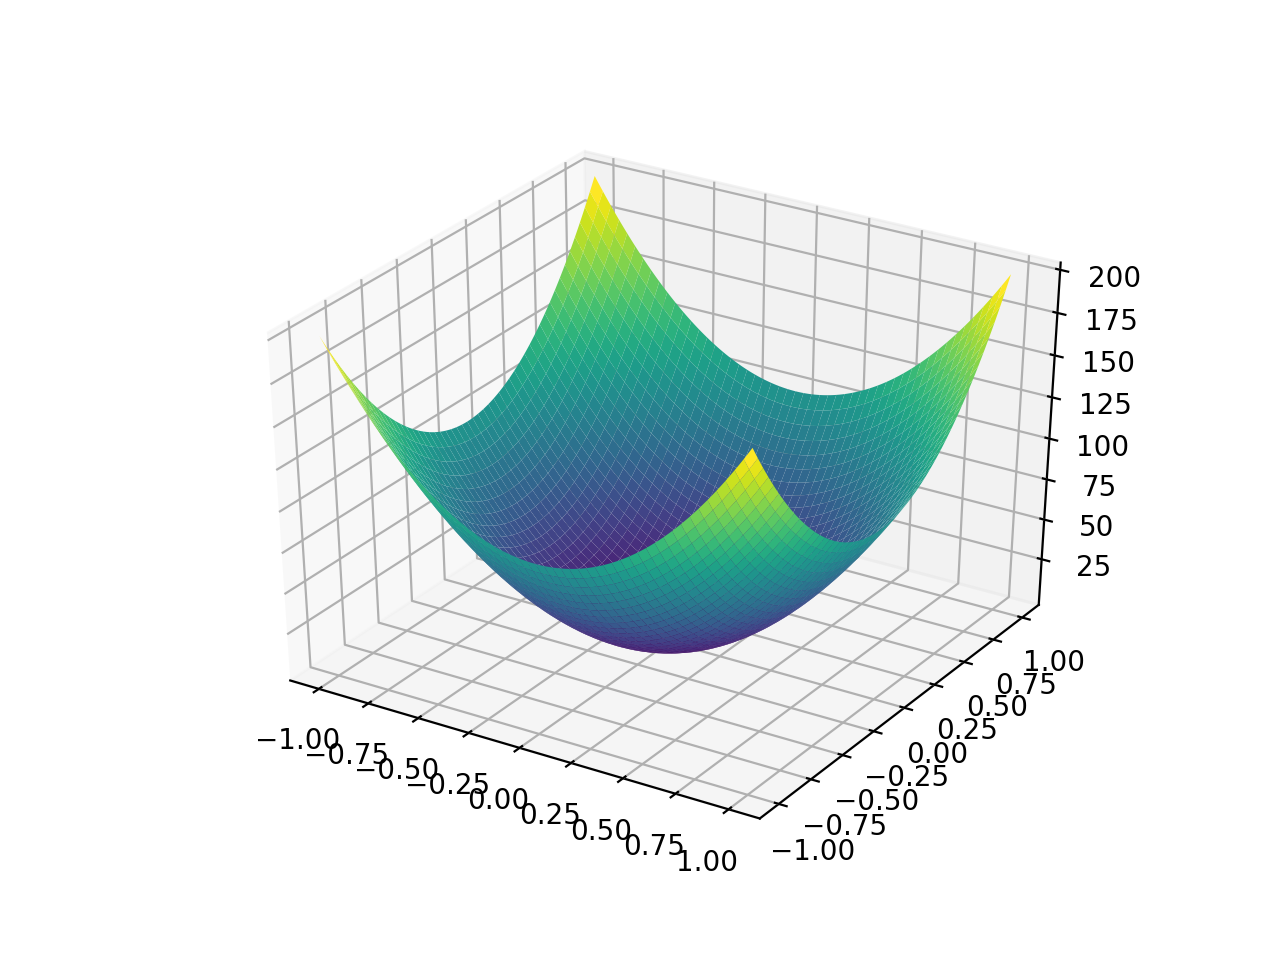
\includegraphics[width=6in]{img/easy-surface.png}
         \caption{Easy test optimization function.}
         \label{fig:surface}
       \end{figure}

    \begin{enumerate}
      \item (Full) Gradient Descent (GD) vs Stochastic \\
        Our experiment validated the hypothesis that stochastic gradient descent
        was faster than gradient descent (about 12x speedup per iteration);
        although the method suffered from its randomness and actually took about
        the same time to converge (quantitative analysis is omitted due to the
        arbitrary nature of the experiment). In Figure \ref{fig:sgd1} the
        optimization paths are shown on a contour of the original function. The
        same learning rate is used, and it is easily seen that the stochastic
        nature actually harms the rate of convergence due to the lack of
        contribution of every term in the sum.
       \begin{figure}[h!]
         \centering
         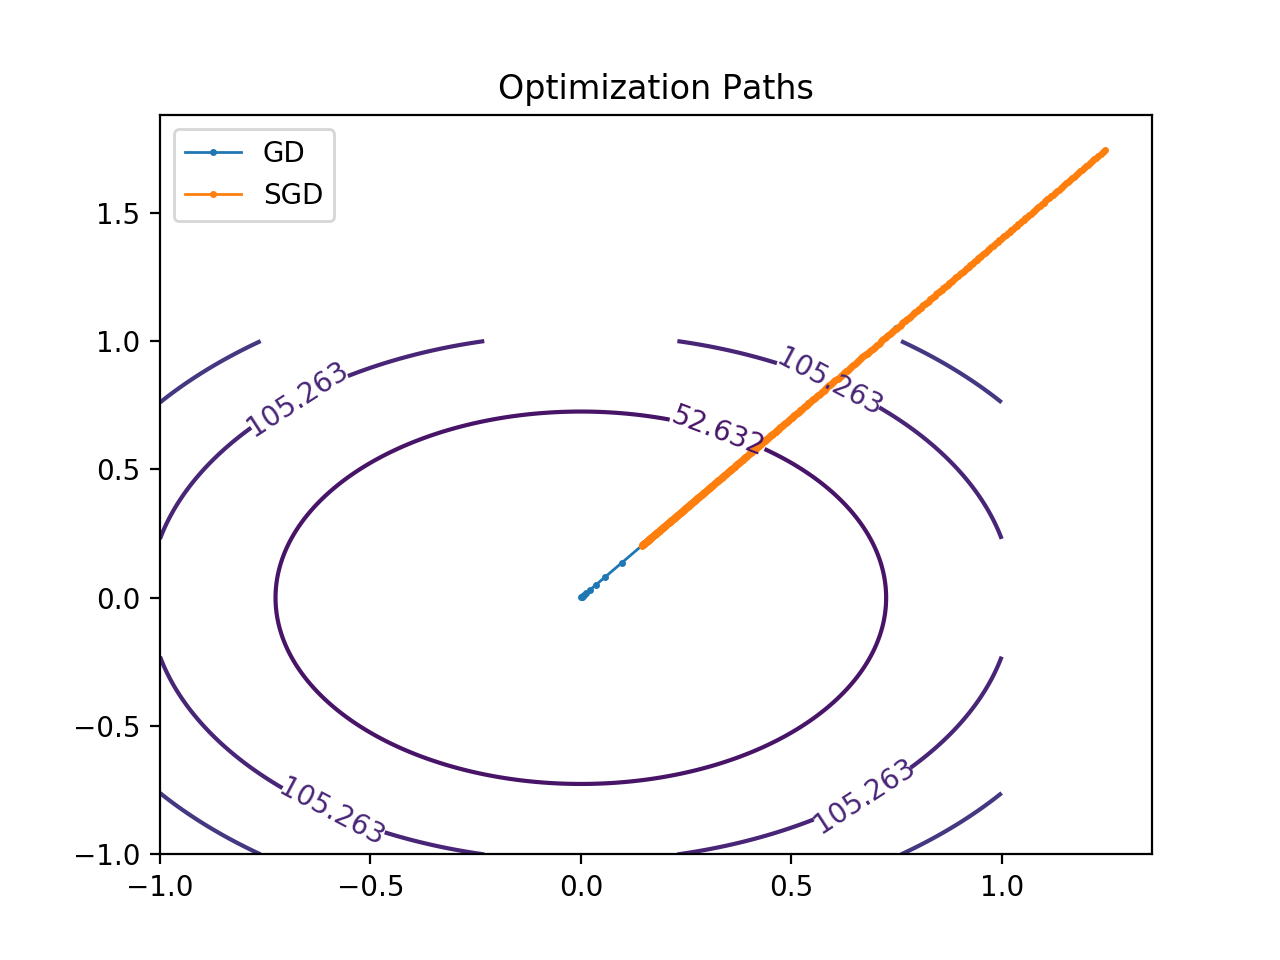
\includegraphics[width=6in]{img/gd-sgd.png}
         \caption{Gradient Descent and SGD optimization paths.}
         \label{fig:sgd1}
       \end{figure}

       \begin{figure}[h!]
         \centering
         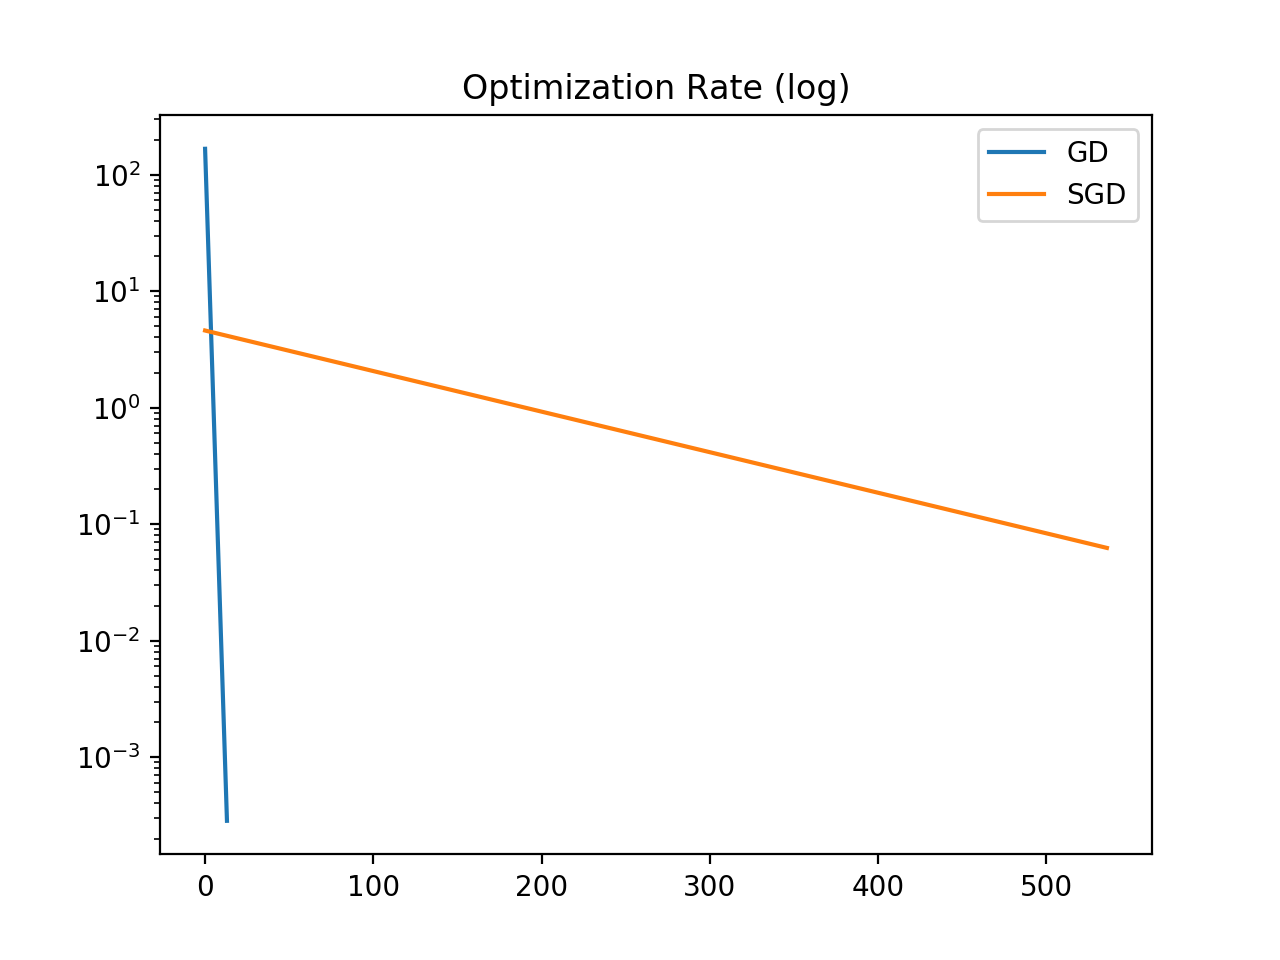
\includegraphics[width=6in]{img/gd-sgd2.png}
         \caption{Gradient Descent and SGD optimization iterations.}
         \label{fig:sgd2}
       \end{figure}

       \begin{figure}[h!]
         \centering
         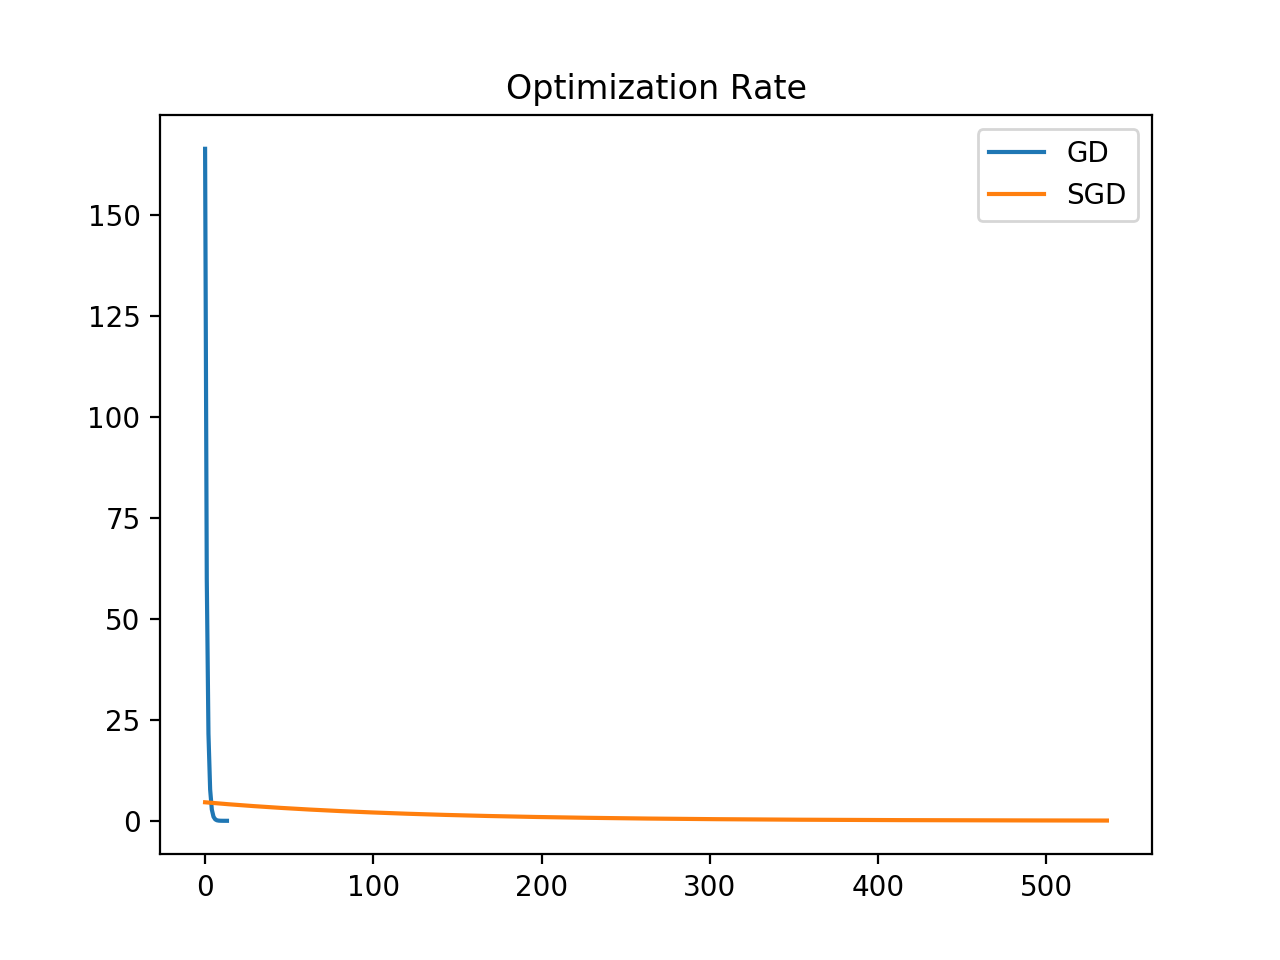
\includegraphics[width=6in]{img/gd-sgd3.png}
         \caption{Gradient Descent and SGD optimization iterations.}
         \label{fig:sgd3}
       \end{figure}

        \FloatBarrier
      \item Stochastic Gradient Descent (SGD) vs Momentum \\
        Whereas the above SGD proved to perform significantly worse than GD in
        order to achieve a speedup, adding a momentum term allowed for both
        faster iteration as in the case of SGD, but also better convergence.

       \begin{figure}[h!]
         \centering
         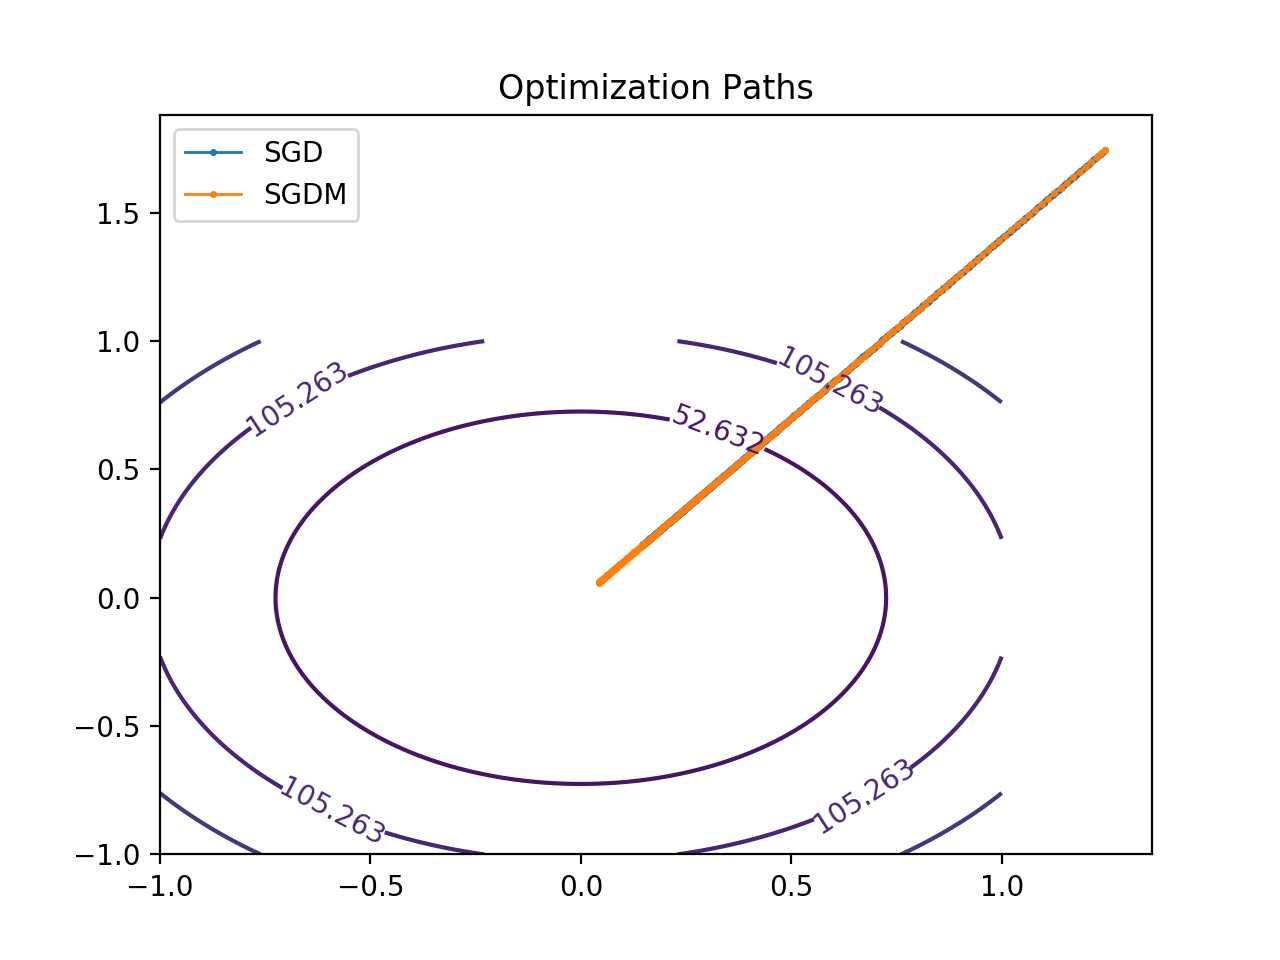
\includegraphics[width=6in]{img/sgdm.png}
         \caption{SGD and SGDM optimization paths.}
         \label{fig:sgdm}
       \end{figure}

       \begin{figure}[h!]
         \centering
         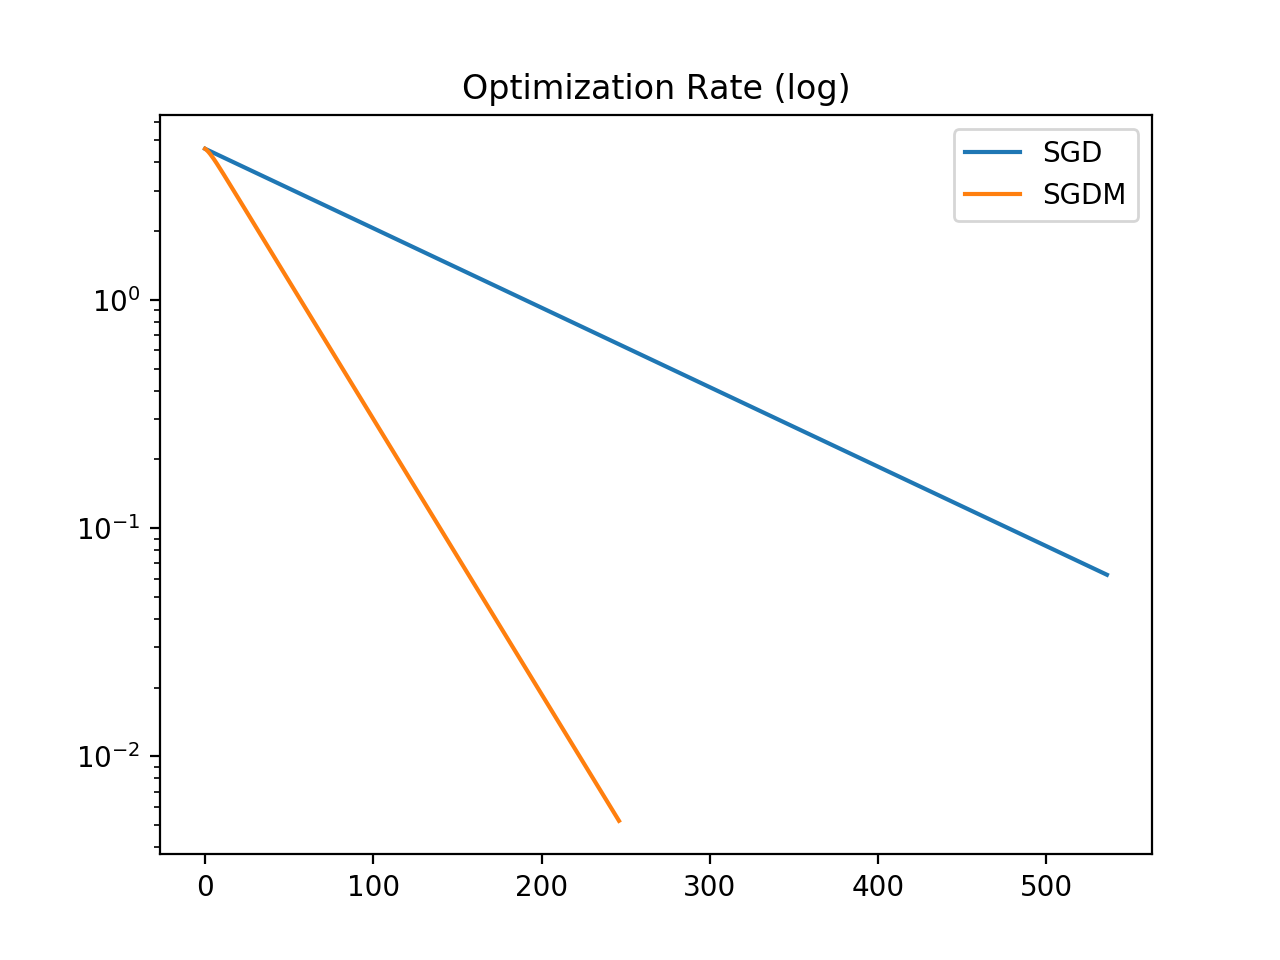
\includegraphics[width=6in]{img/sgdm2.png}
         \caption{SGD and SGDM optimization iterations.}
         \label{fig:sgdm2}
       \end{figure}

       \begin{figure}[h!]
         \centering
         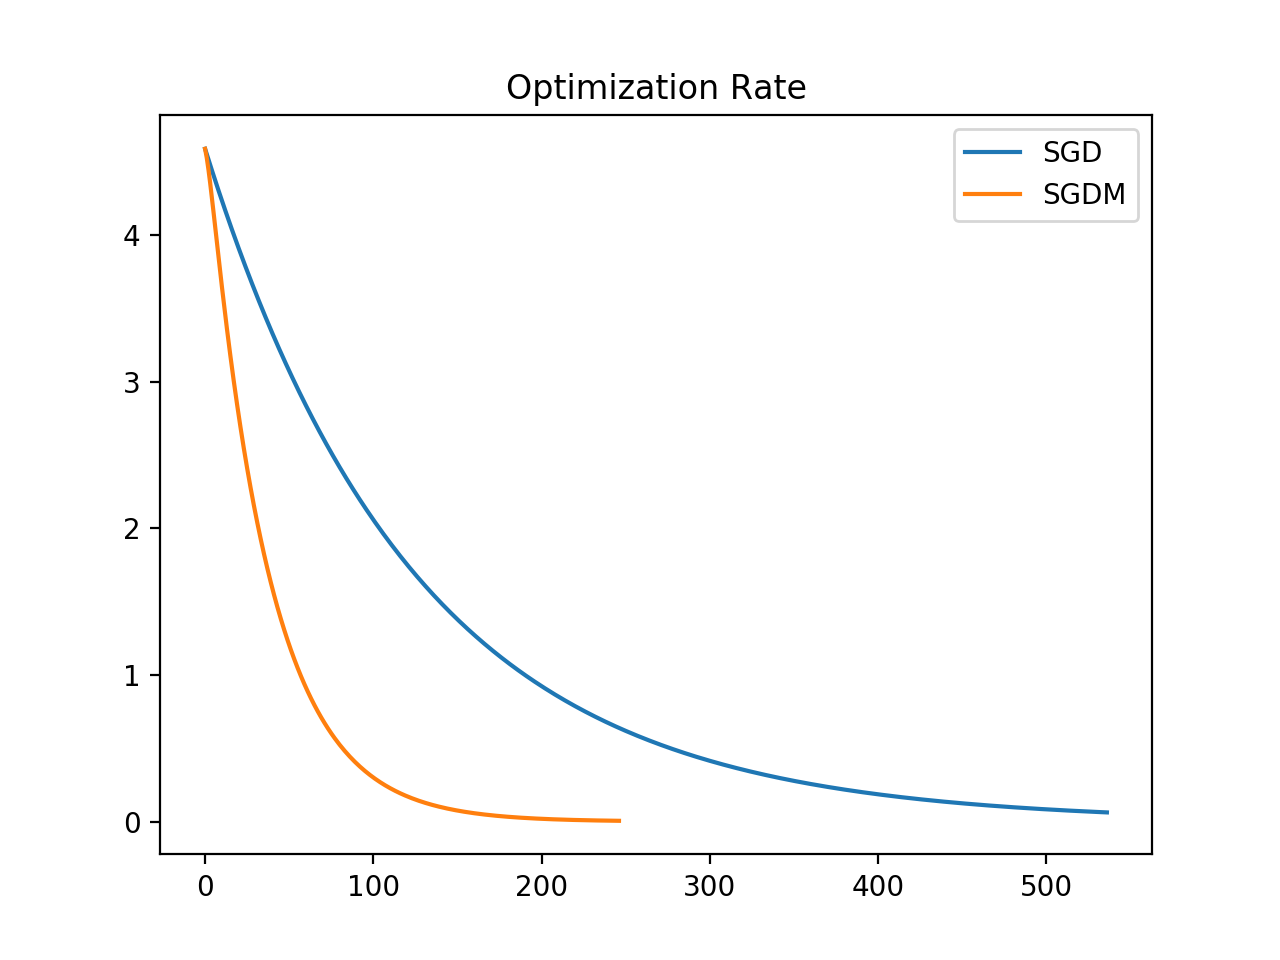
\includegraphics[width=6in]{img/sgdm3.png}
         \caption{SGD and SGDM optimization iterations.}
         \label{fig:sgdm3}
       \end{figure}

        \FloatBarrier
      \item Momentum anti-pattern \\
        As momentum introduces a new hyperparameter, $\alpha$, there are cases
        when it will perform significantly worse than SGD. Below illustrates
        such a case where the learning rate was set to .005 and the momentum was
        set too high at .9.

        \begin{figure}[h!]
         \centering
         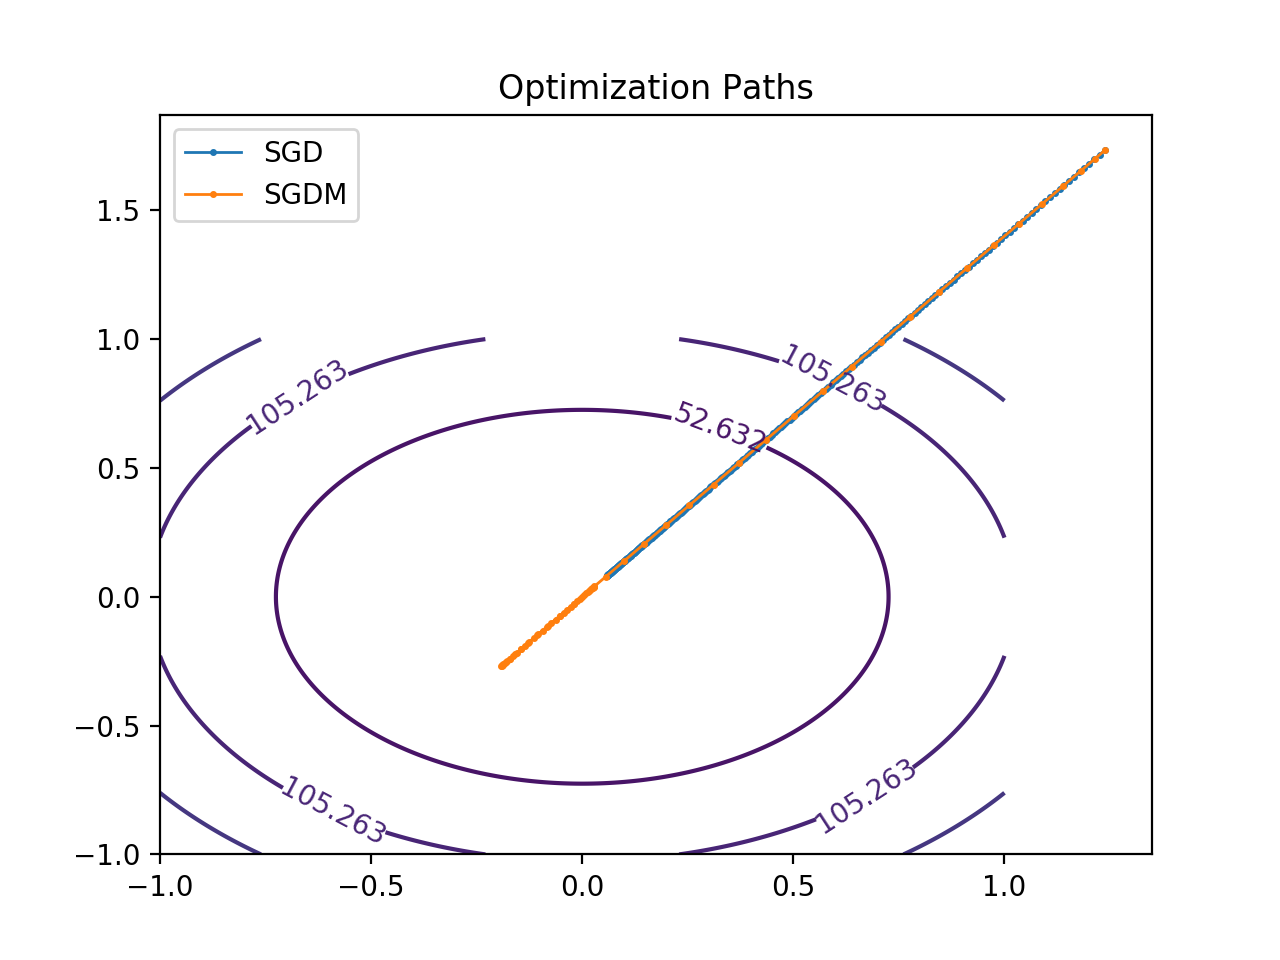
\includegraphics[width=6in]{img/bad_momentum.png}
         \caption{Poor momentum selection paths.}
         \label{fig:sgdm}
       \end{figure}

       \begin{figure}[h!]
         \centering
         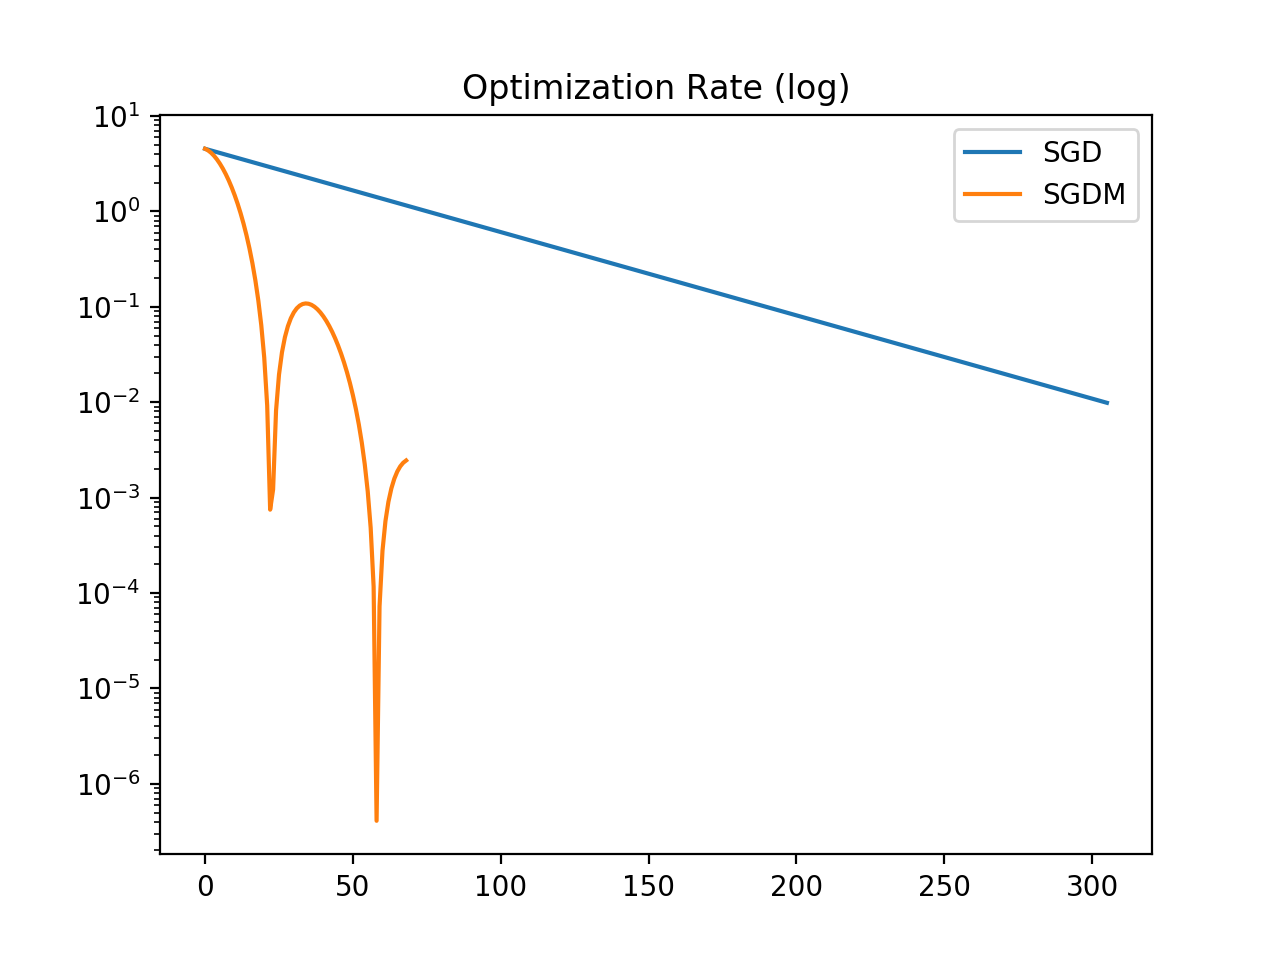
\includegraphics[width=6in]{img/bad_momentum2.png}
         \caption{Poor momentum selection optimization iterations.}
         \label{fig:sgdm2}
       \end{figure}

       \begin{figure}[h!]
         \centering
         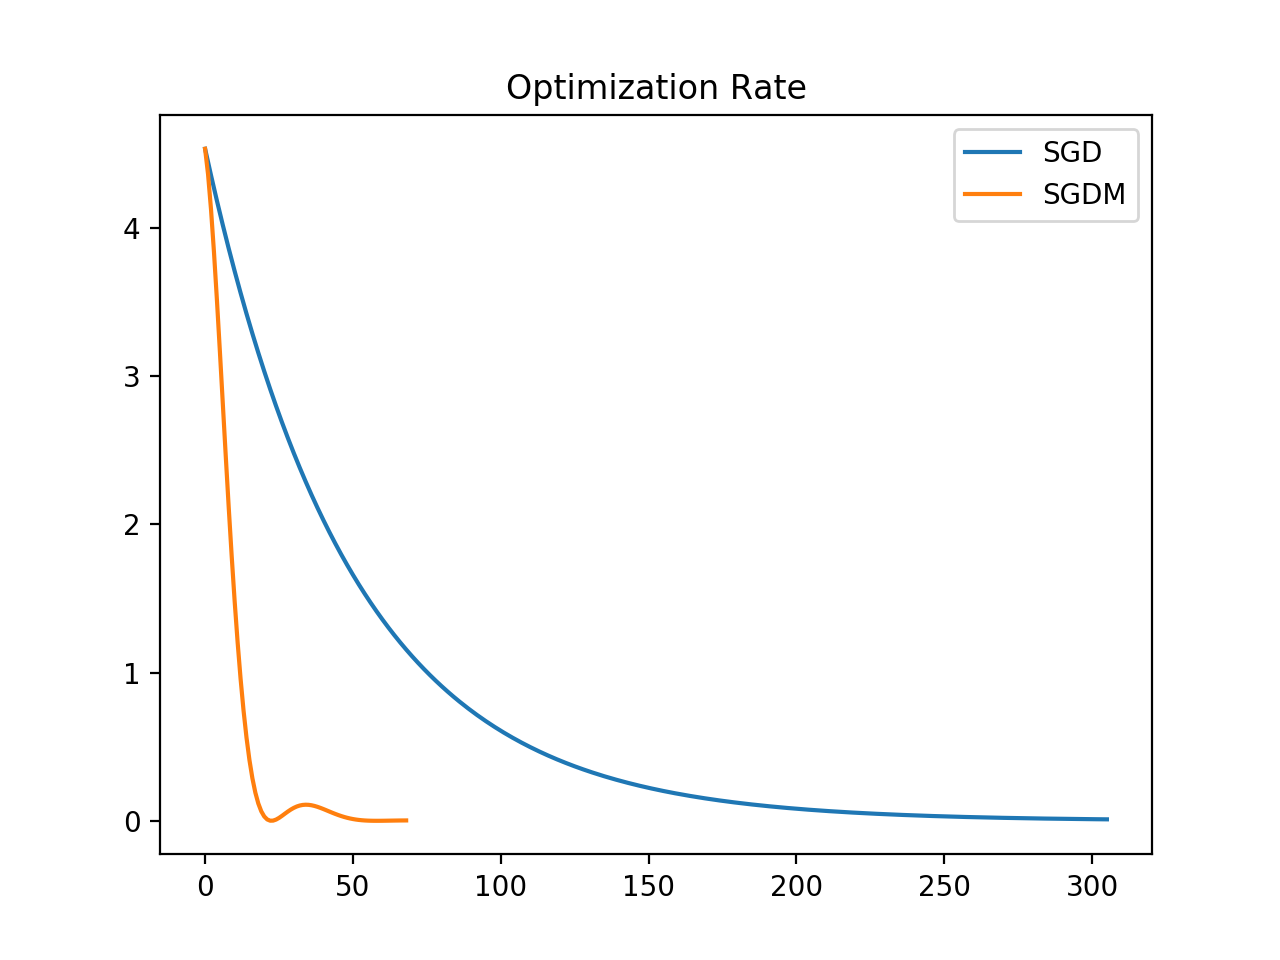
\includegraphics[width=6in]{img/bad_momentum3.png}
         \caption{Poor momentum selection optimization iterations.}
         \label{fig:sgdm3}
       \end{figure}

        \FloatBarrier
      \item Batching \\
        Batching in each test provided expected results, greater convergence
        rate and slightly longer optimization times.
       
        \begin{figure}[h!]
         \centering
         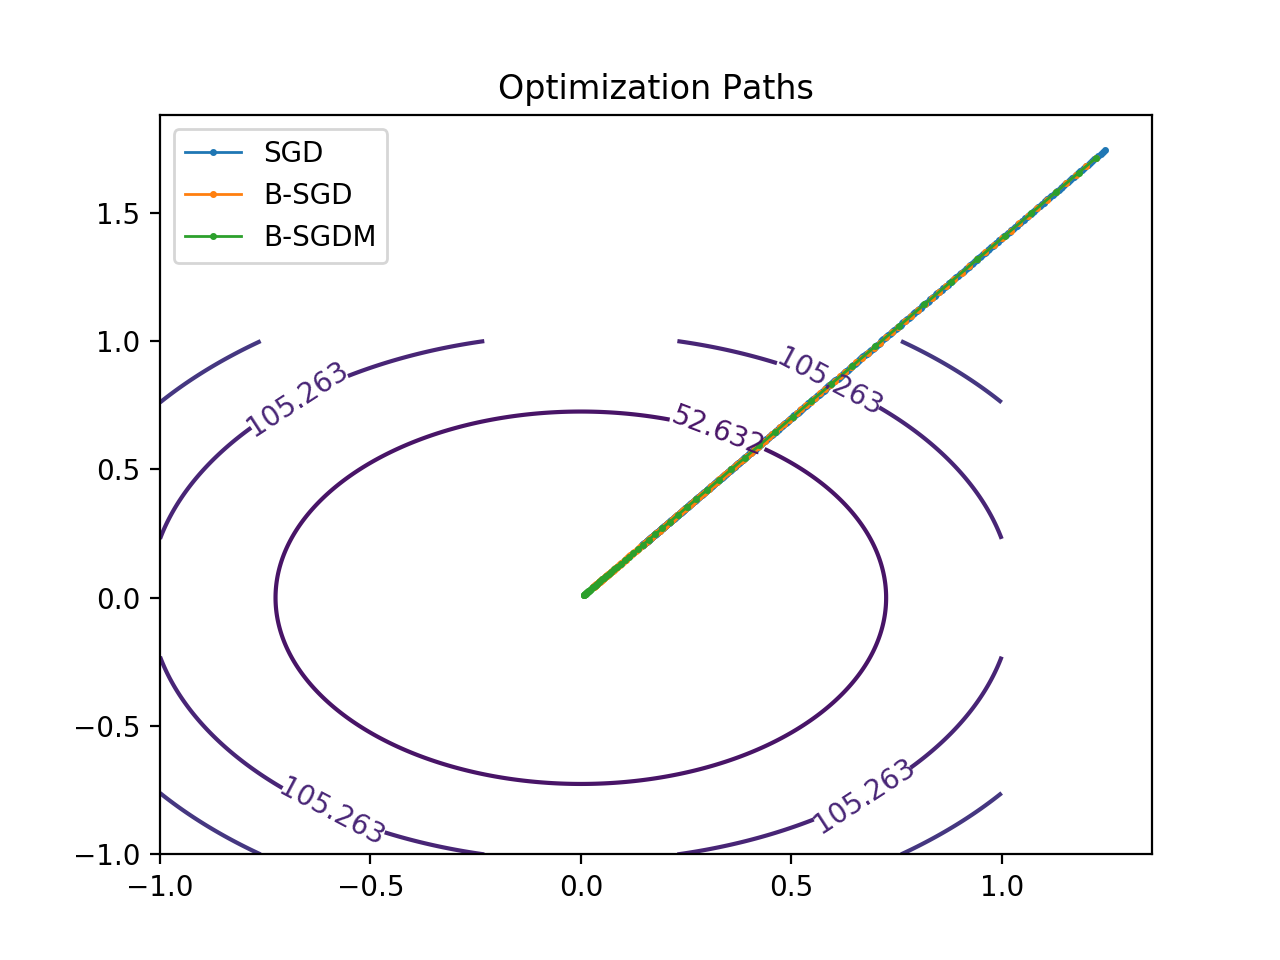
\includegraphics[width=6in]{img/batch.png}
         \caption{SGD vs Batching SGD and Batching SGDM}
         \label{fig:sgdm}
       \end{figure}

       \begin{figure}[h!]
         \centering
         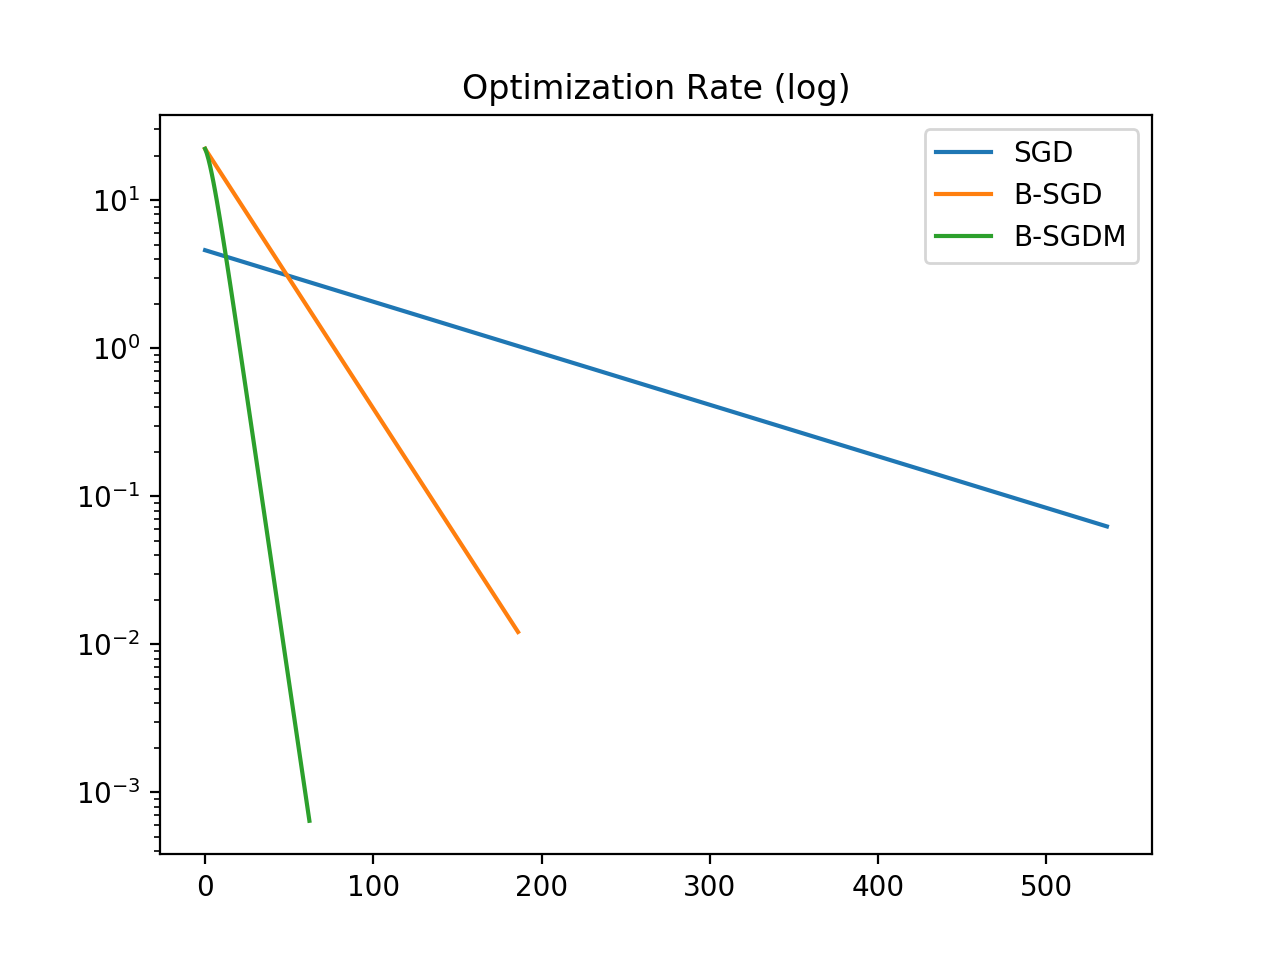
\includegraphics[width=6in]{img/batch2.png}
         \caption{SGD vs Batching SGD and Batching SGDM}
         \label{fig:sgdm2}
       \end{figure}

       \begin{figure}[h!]
         \centering
         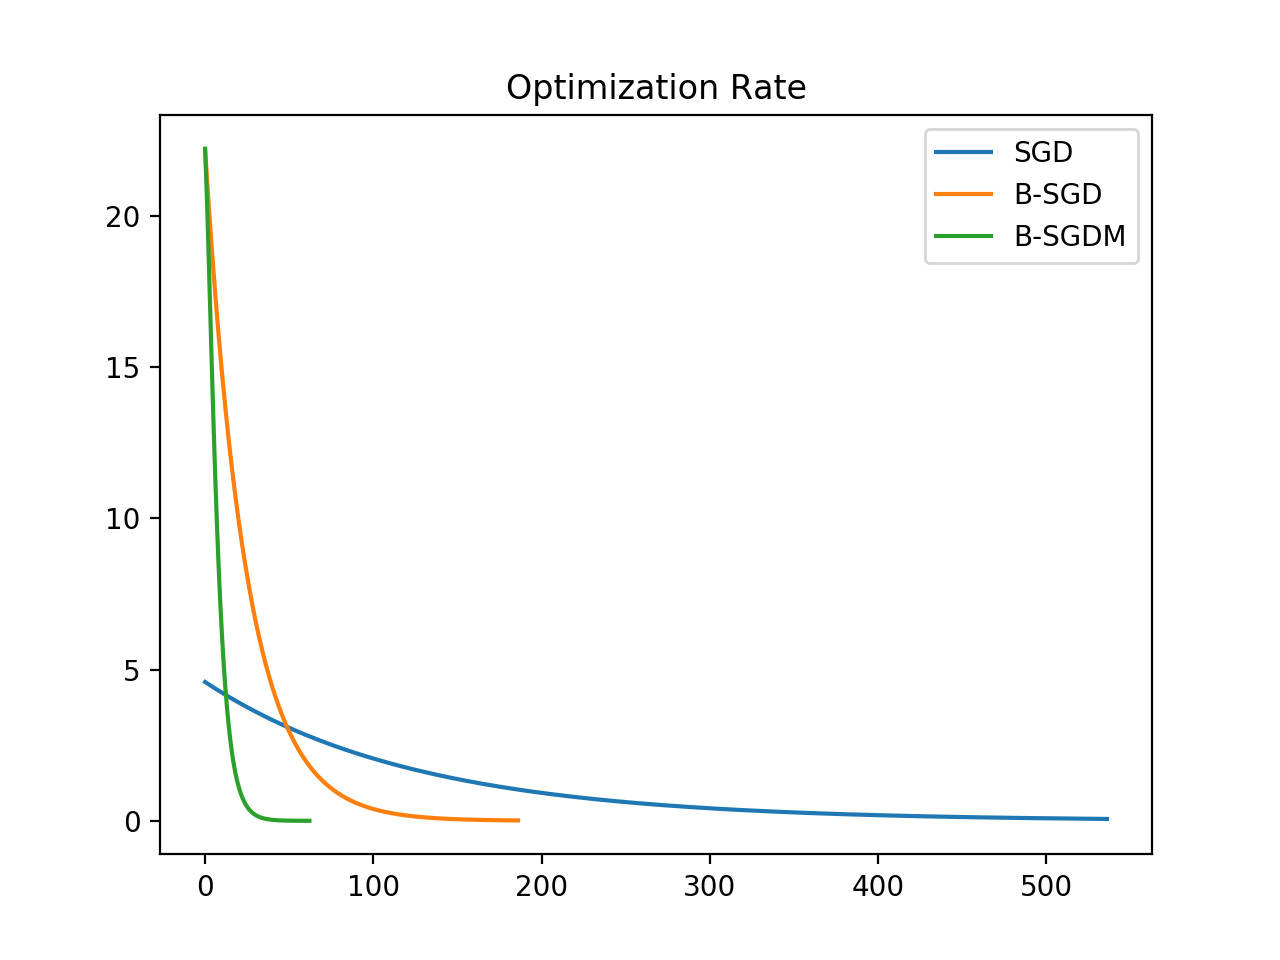
\includegraphics[width=6in]{img/batch3.png}
         \caption{SGD vs Batching SGD and Batching SGDM}
         \label{fig:sgdm3}
       \end{figure}

         \begin{figure}[h!]
         \centering
         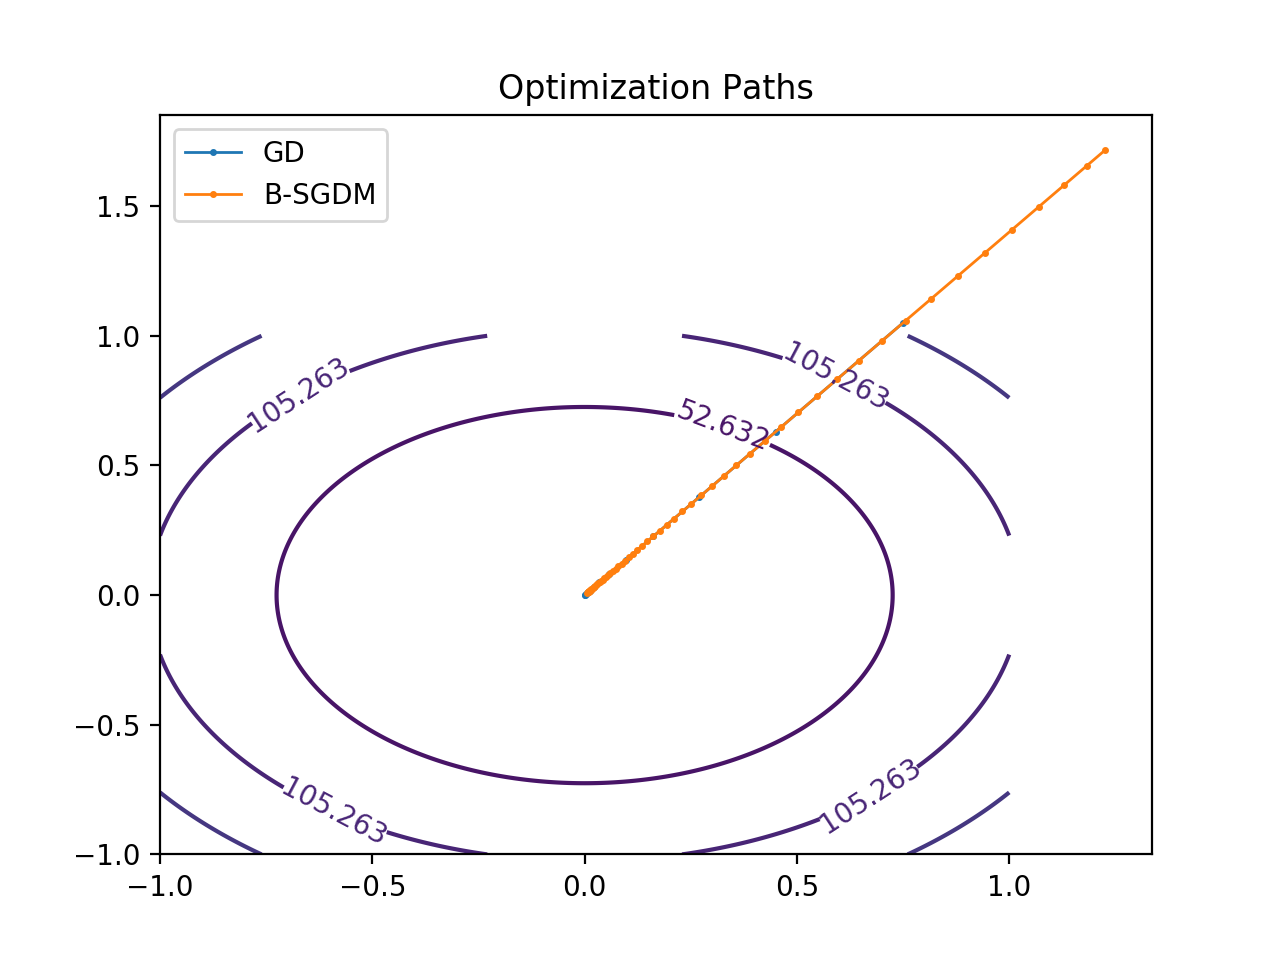
\includegraphics[width=6in]{img/gd-batch.png}
         \caption{GD vs Batching SGDM}
         \label{fig:sgdm}
       \end{figure}

       \begin{figure}[h!]
         \centering
         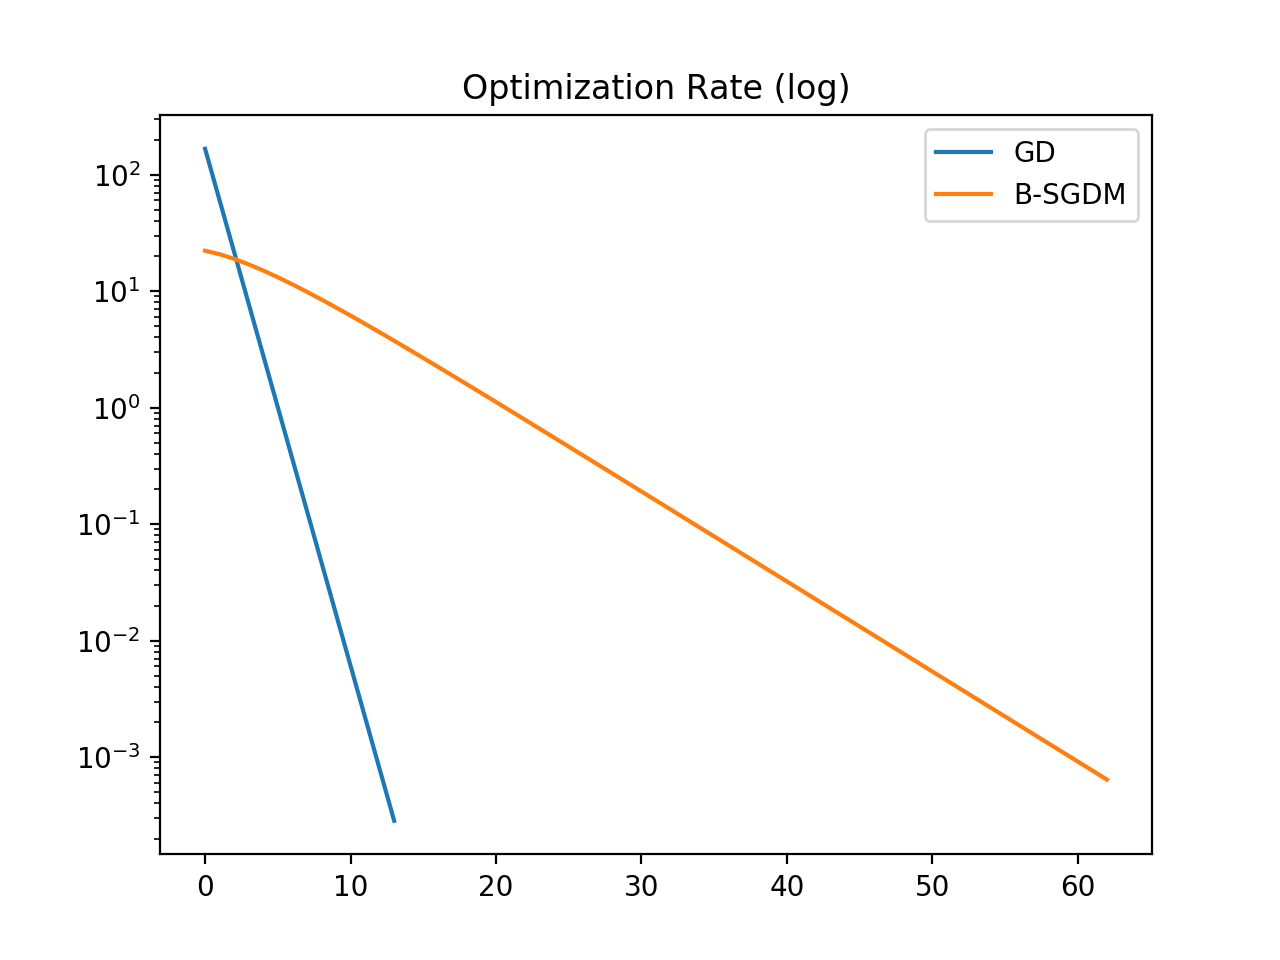
\includegraphics[width=6in]{img/gd-batch2.png}
         \caption{GD vs Batching SGDM}
         \label{fig:sgdm2}
       \end{figure}

       \begin{figure}[h!]
         \centering
         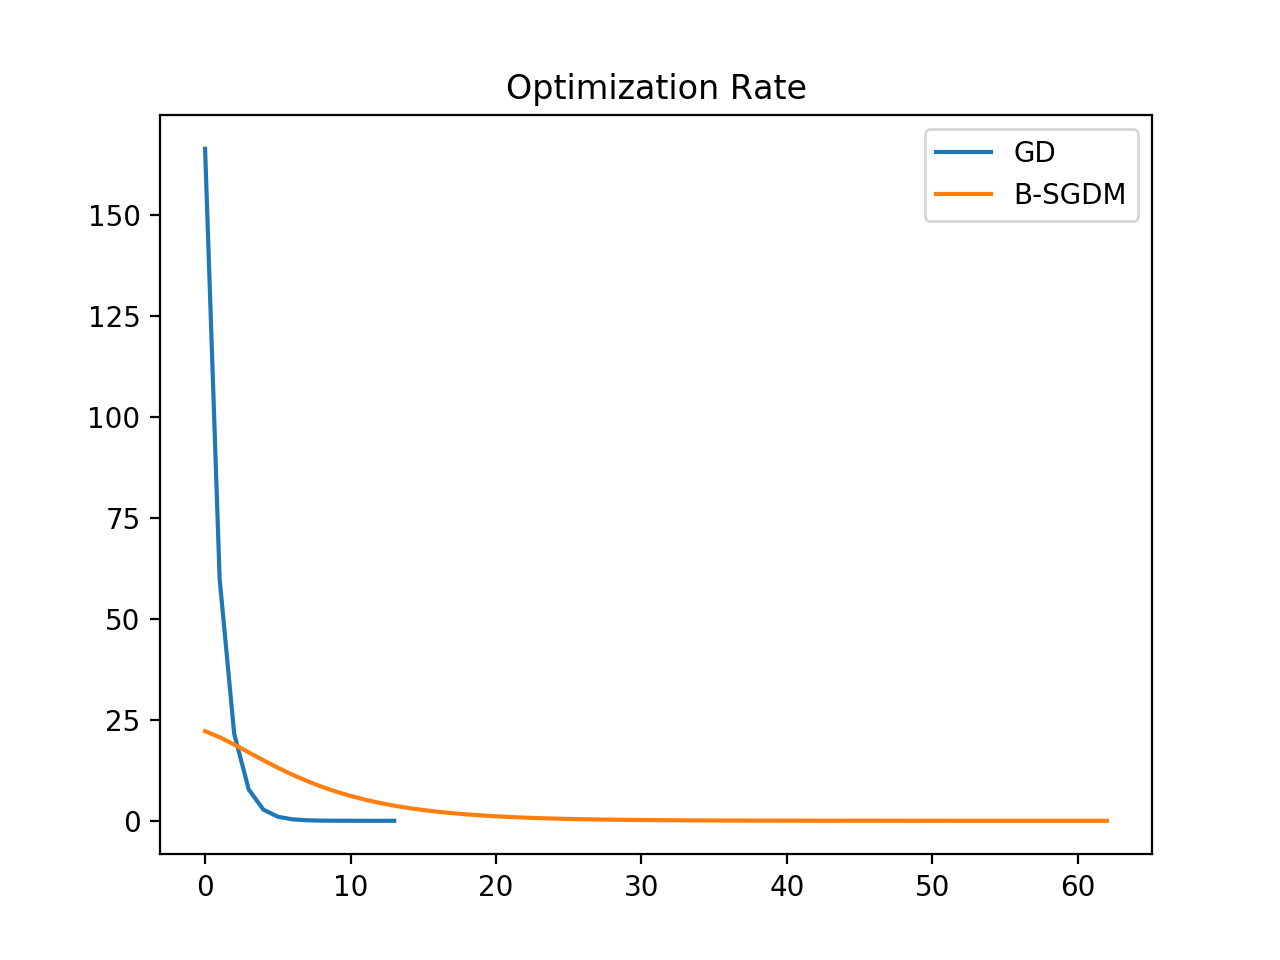
\includegraphics[width=6in]{img/gd-batch3.png}
         \caption{GD vs Batching SGDM}
         \label{fig:sgdm3}
       \end{figure}

        \FloatBarrier
      \item Adaptive Methods \\
        The adaptive methods provided more robust optimization although were not
        necessarily exhibited well in this simple convex function. See below for
        a better use-case.
       
        \begin{figure}[h!]
         \centering
         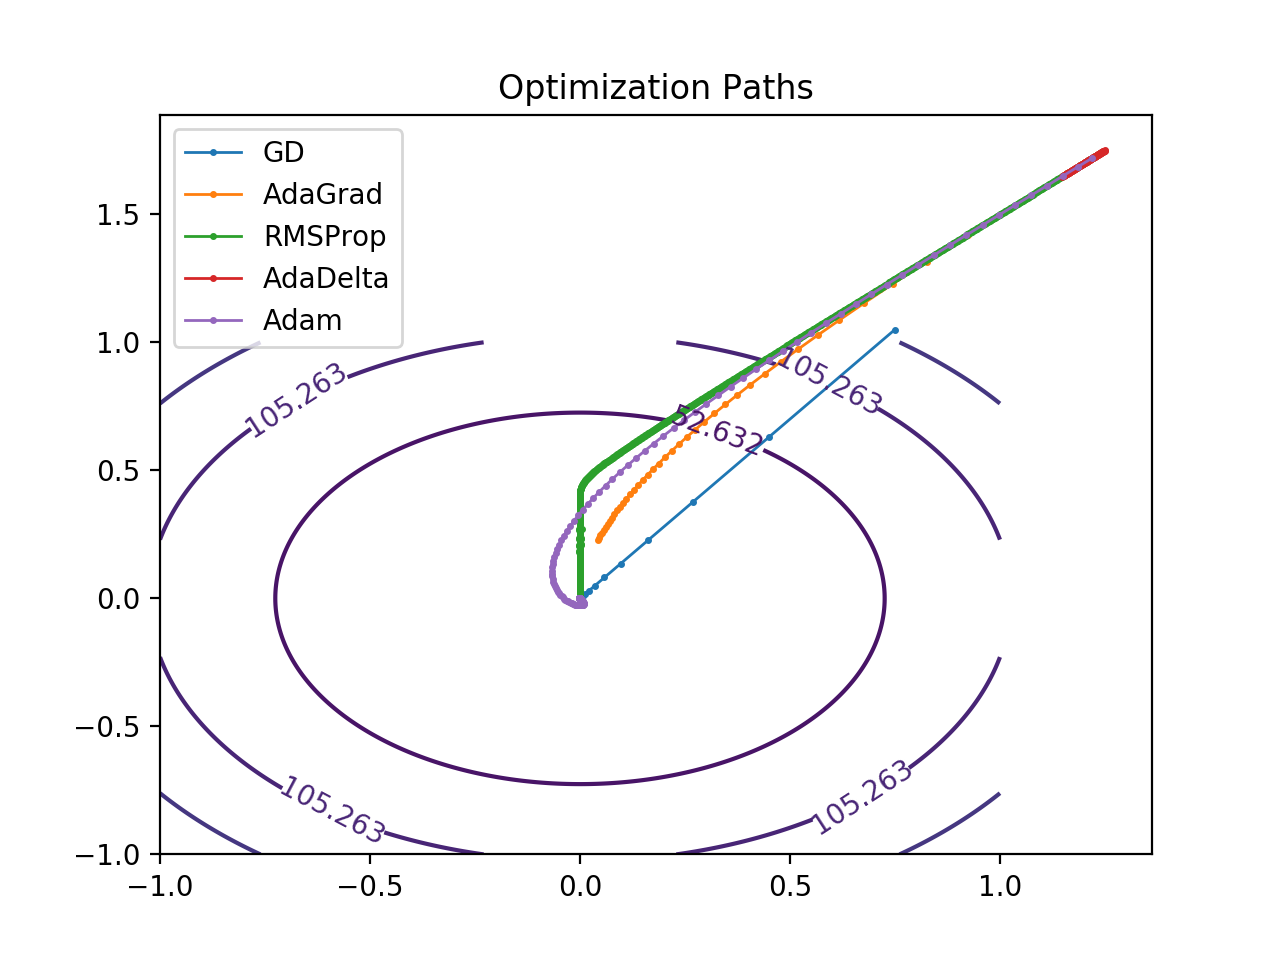
\includegraphics[width=6in]{img/adas.png}
         \caption{Adaptive methods optimization paths.}
         \label{fig:sgdm}
       \end{figure}

       \begin{figure}[h!]
         \centering
         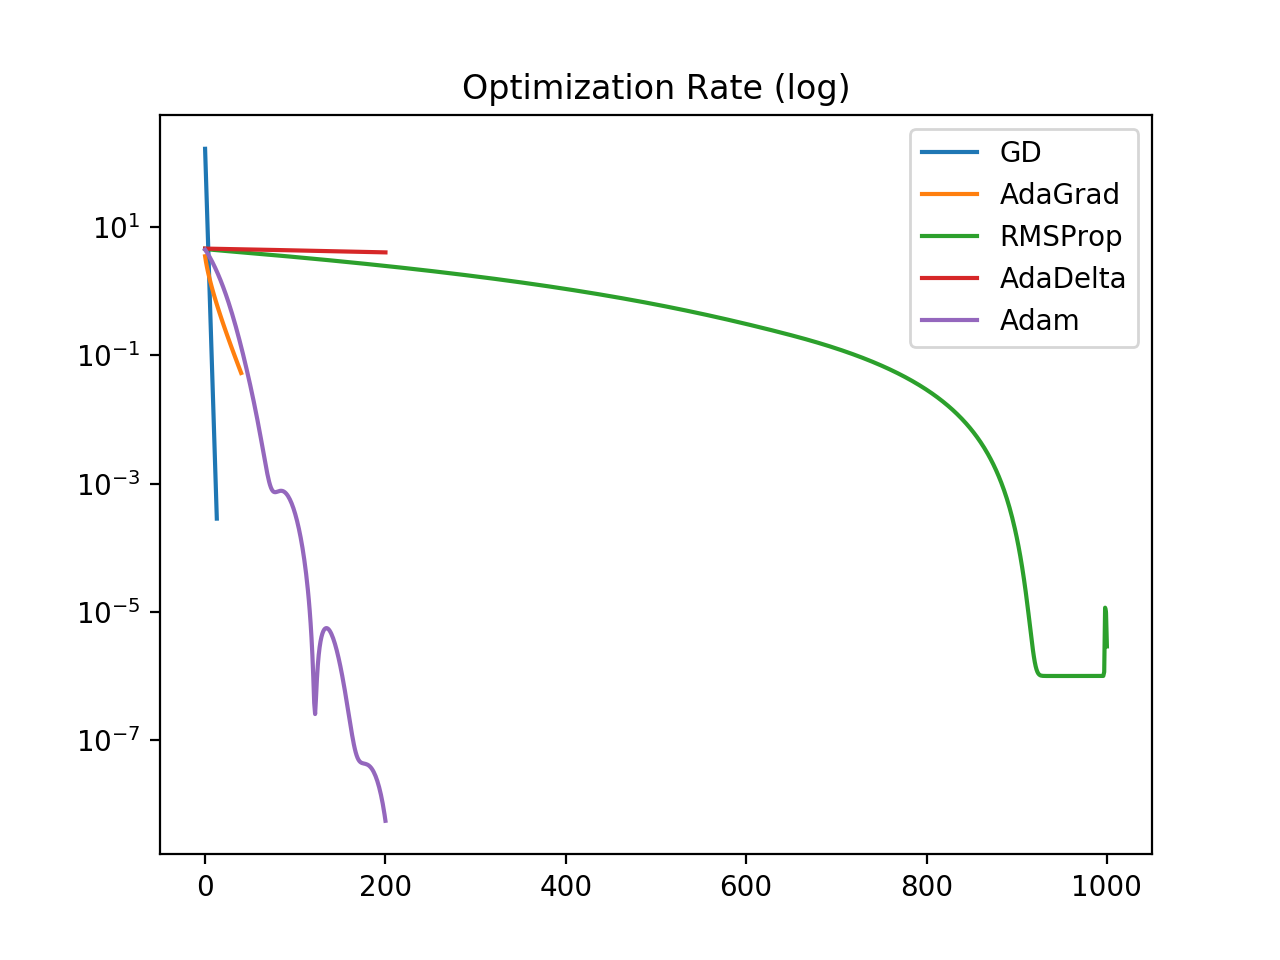
\includegraphics[width=6in]{img/adas2.png}
         \caption{Adaptive methods optimization iterations.}
         \label{fig:sgdm2}
       \end{figure}

       \begin{figure}[h!]
         \centering
         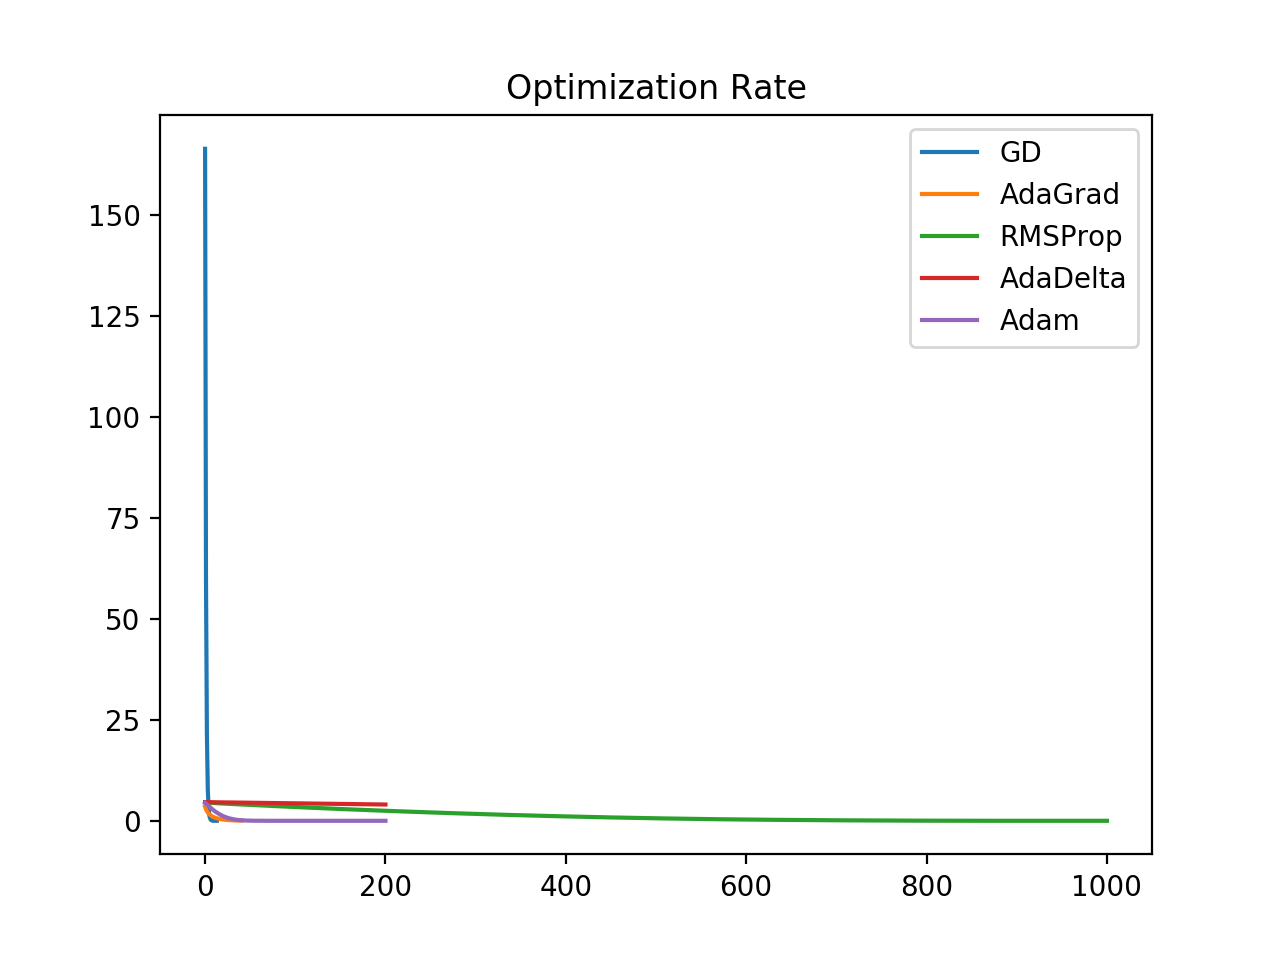
\includegraphics[width=6in]{img/adas3.png}
         \caption{Adaptive methods optimization iterations.}
         \label{fig:sgdm3}
       \end{figure}


        \FloatBarrier
      \item Non-convex Function \\
        To test how many of these methods react to a more difficult optimization
        function (akin to what would be encountered in real-world data), we
        simulated the following non-convex function:
        \[
        f(x, y) = 1 - e^{-(10x^{2}+y^{2})}
        \]

        In general, our results were what we expected: Adam performed the best
        and was capable of optimization while nearly all the others couldn't.

        \begin{figure}[h!]
         \centering
         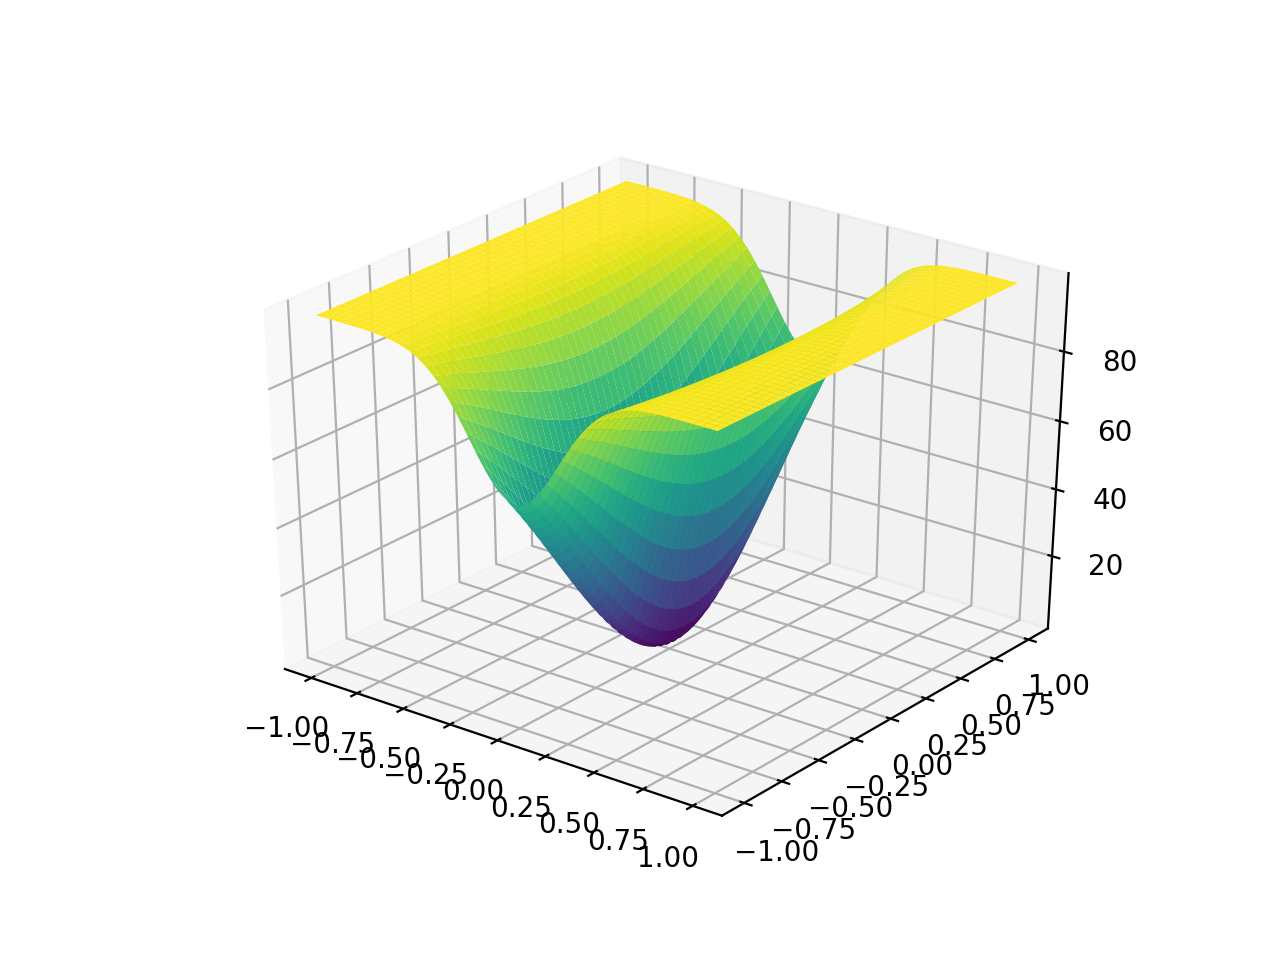
\includegraphics[width=6in]{img/hard-surface.png}
         \caption{Non-convex optimization function.}
         \label{fig:hard-surface}
       \end{figure}

        \begin{figure}[h!]
         \centering
         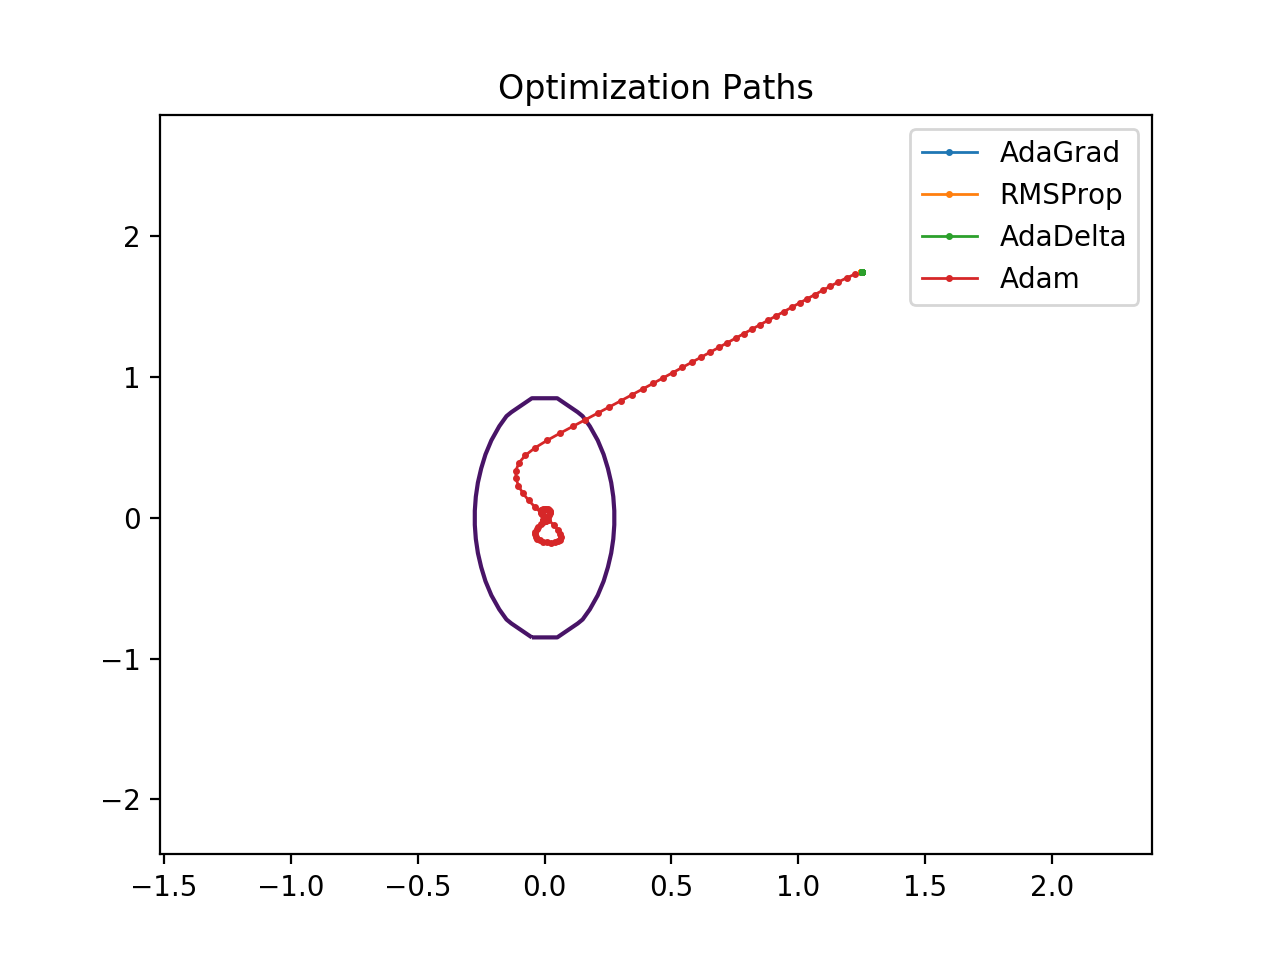
\includegraphics[width=6in]{img/hard.png}
         \caption{Non-convex optimization function paths.}
         \label{fig:sgdm}
       \end{figure}

       \begin{figure}[h!]
         \centering
         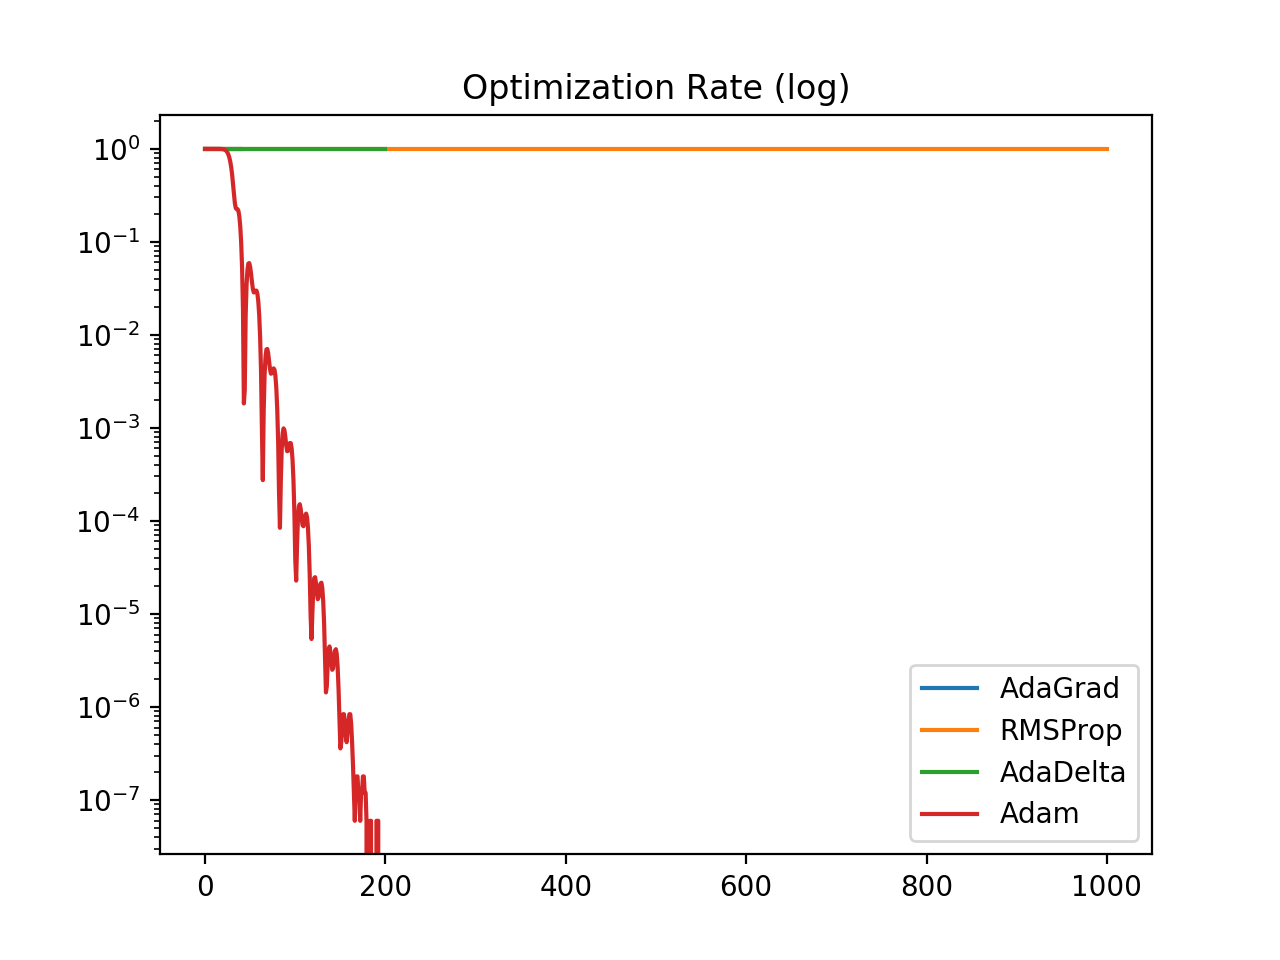
\includegraphics[width=6in]{img/hard2.png}
         \caption{Non-convex optimization function iterations.}
         \label{fig:sgdm2}
       \end{figure}

       \begin{figure}[h!]
         \centering
         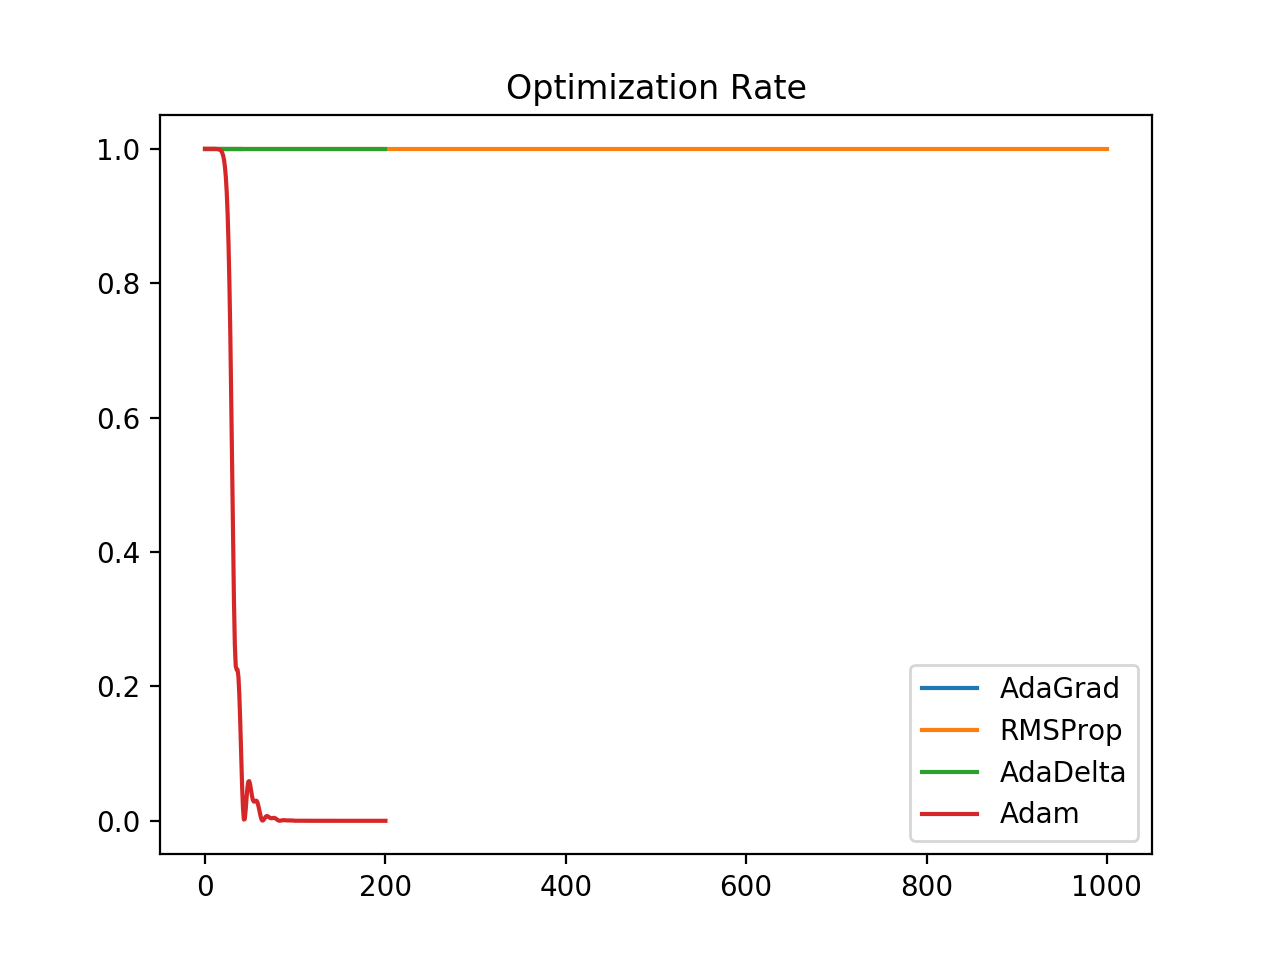
\includegraphics[width=6in]{img/hard3.png}
         \caption{Non-convex optimization function iterations.}
         \label{fig:sgdm3}
       \end{figure}
       
    \end{enumerate}

\end{enumerate}

\FloatBarrier

\section*{Problem 6: Perceptron case study}

\begin{enumerate}[\bf (i)]

\item We implemented the 3 versions of Perceptron first as binary classifiers, and then extended to a multiclass case using one-versus-all comparison. To double check our work, we ran synthetic, 2-class data through both the binary and extended multiclass versions, and for each version of Perceptron, we got exactly matching results between the binary and multiclass implementations. We then applied these algorithms to the MNIST dataset.

\item A three-fold cross-validation analysis was done of the three Perceptron versions at various maximum iterations (values of T). At very low values of T, all three versions of Perceptron are comparably bad (though still better than random guessing, which would have an accuracy of approximately 0.1). As the value of T increases, Perceptron V2 emerges as the most effective classifier for this MNIST task, followed by V0, and finally by V1. \\
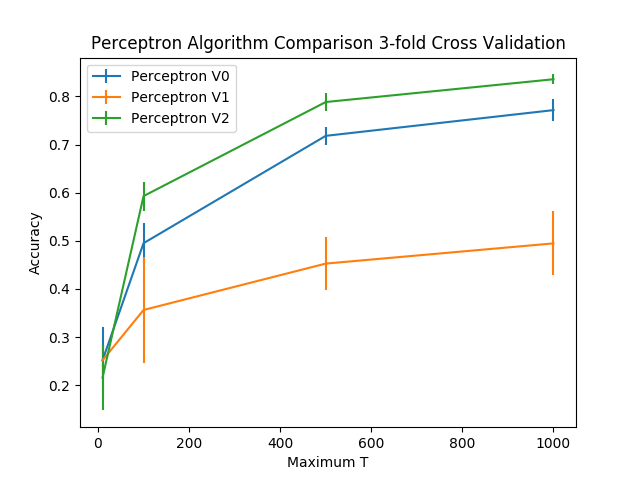
\includegraphics[width=0.8\textwidth]{perceptron_compare.png}\\
A similar 3-fold cross-validation experiment was done with different sized training sets. In this experiment, Perceptron V1 and Perceptron V2 performed comparably, and both outperformed V0.\\
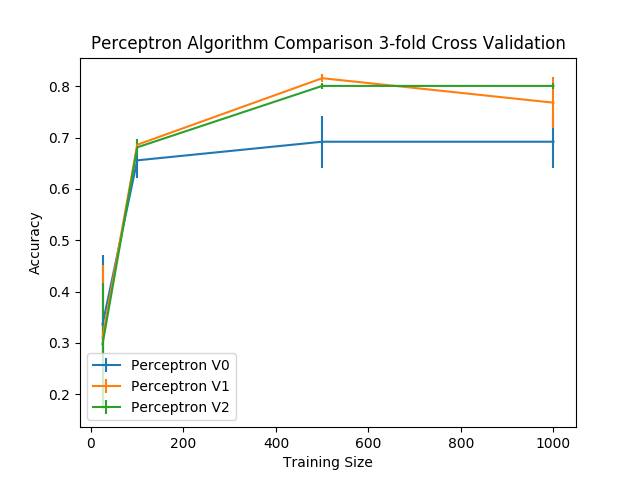
\includegraphics[width=0.8\textwidth]{perceptron_compare_size.png}

\item For the Kernel Perceptron, we once again turned to a synthetic binary dataset to ensure that our binary and multi-class implementations were working as expected. On our synthetic set, the performance was:
\\
\begin{tabular}{|c|c|c|}
	\hline
	\textbf{Perceptron} & \textbf{Binary Accuracy} & \textbf{``Multiclass'' Accuracy}\\ \hline
	V0 & 0.724 & 0.724 \\
	V1 & 0.632 & 0.632 \\
	V2 & 0.736 & 0.736 \\
	Kernel & 0.748 & 0.748 \\ \hline
\end{tabular}
\\
The fact that our implementations have matching performace on a two-class problem for both the base and multi-class implementations show that the multi-class extension is implemented correctly. As expected, the Kernel Perceptron is the best performer. When we generated the synthetic data, we intentionally set it to NOT be linearly separable. Thus, the Kernel version probably improves performance because the data is separable in a transformed space. For completeness, we also tested true multi-class (5 class) data through the implementations:
\\
\begin{tabular}{|c|c|}
	\hline
	\textbf{Perceptron} & \textbf{Multiclass Accuracy}\\ \hline
	V0 & 0.376  \\
	V1 & 0.192  \\
	V2 & 0.384  \\
	Kernel & 0.456\\ \hline
\end{tabular}
\\
We, once again, see that the Kernel version is the top performer.
\end{enumerate}

\end{document} 
